\documentclass[a4paper, 11pt, accentcolor = tud3b]{tudreport}

% Core packages.
\usepackage[T1]{fontenc}
\usepackage[utf8]{inputenc}
\usepackage[ngerman]{babel}
% Other packages.
\usepackage{caption}
\usepackage{csquotes}
\usepackage{enumitem}
\usepackage[mathcal]{euscript} % Get readable mathcal font.
\usepackage{float}
\usepackage{hyperref}
\usepackage{mathtools}
\usepackage{siunitx}
\usepackage{stmaryrd}
\usepackage{tabto}
\usepackage{tikz}
\usepackage[disable]{todonotes}
\usetikzlibrary{arrows.meta, shapes, backgrounds, angles, calc, decorations.markings}

% Basic information.
\title{Grundlagen der Robotik}
\subtitle{Zusammenfassung \\ Fabian Damken}
\author{Fabian Damken}
\date{\today}

% Description-list styling.
\SetLabelAlign{parright}{\parbox[t]{\labelwidth}{\raggedleft#1}}
\setlist[description]{style = multiline, leftmargin = 4cm, align = parright}

\tikzset{> = { Latex[length = 2.5mm] }}
\tikzstyle{every path} = [ very thick ]

% New commands.
\DeclareMathOperator{\total}{d}
\newcommand{\dif}[1]{\,\total#1}
% Matrix/Vector notation.
\newcommand{\mat}[1]{\boldsymbol{\mathbf{#1}}}
\renewcommand{\vec}[1]{\boldsymbol{\mathbf{#1}}}
% Abbreviations.
\renewcommand{\dh}{d.\,h.~}
\newcommand{\bzw}{bzw.~}
\newcommand{\bspw}{bspw.~}
\newcommand{\bzgl}{bzgl.~}
\newcommand{\zB}{z.\,B.~}
\newcommand{\iA}{i.\,A.~}
\newcommand{\ggf}{ggf.~}

% https://tex.stackexchange.com/a/333383
\makeatletter
\renewcommand*\env@matrix[1][*\c@MaxMatrixCols c]{%
	\hskip -\arraycolsep
	\let\@ifnextchar\new@ifnextchar
	\array{#1}}
\makeatother

\begin{document}
	\maketitle
	\tableofcontents
	\listoftodos

	\chapter{Einleitung} % 1.8
		\todo{Content}
		
		\section{Was ist ein Roboter?} % 1.9, 1.10, 1.11, 1.12, 1.13, 1.14
			\todo{Content}
		% end

		\section{Was ist KI?} % 1.15, 1.16, 1.17, 1.18, 1.19
			\todo{Content}
		% end

		\section{Was ist Robotik?} % 1.20, 1.21, 1.22
			\todo{Content}
		% end

		\section{Sense -- Plan -- Act} % 1.27
			\todo{Content}

			\paragraph{Act} % N/A
				\todo{Content}

				\subparagraph{Kinematik} % 1.28, 1.29, 1.30, 1.31, 2.32, 1.33, 1.34, 1.35
					\todo{Content}
				% end

				\subparagraph{Dynamik} % 1.36, 1.37
					\todo{Content}
				% end

				\subparagraph{Steuerung} % 1.38, 1.39, 1.40, 1.41
					\todo{Content}
				% end
			% end

			\paragraph{Sense} % N/A
				\todo{Content}

				\subparagraph{Sensoren} % 1.42, 1.43, 1.44, 1.45
					\todo{Content}
				% end
			% end

			\paragraph{Plan} % N/A
				\todo{Content}

				\subparagraph{Lokalisierung, Kartographie, Navigation, Bahnplanung} % 1.46, 1.47, 1.48, 1.49
					\todo{Content}
				% end
			% end
		% end

		\section{Geschichte der Robotik} % 1.50
			\todo{Content}

			\subsection{Historische Entwicklung} % 1.51, 1.54, 1.55
				\todo{Content}
			% end

			\subsection{Die drei Gebote der Robotik} % 1.52, 1.53
				\todo{Content}
			% end

			\subsection{Autonome Fahrzeuge} % 1.59
				\todo{Content}
			% end

			\subsection{Entwicklungstrend} % 1.60
				\todo{Content}
			% end
		% end

		\section{Herausforderungen} % 1.61
			\todo{Content}

			\subsection{Humanoide Bewegung} % 1.61, 1.61, 1.63, 1.64, 1.65, 1.66, 1.67, 1.68, 1.69
				\todo{Content}
			% end

			\subsection{Roboter für menschliche Mobilität} % 1.112, 1.113, 1.114, 1.115, 1.116, 1.117, 1.118, 1.119, 1.120, 1.121, 1.122, 1.123
				\todo{Content}
			% end

			\subsection{Roboter-Avatare} % 1.70
				\todo{Content}

				\subsubsection{Beine} % 1.74, 1.75, 1.76, 1.77, 1.78, 1.79, 1.80, 1.81, 1.82, 1.83, 1.84
					\todo{Content}
				% end

				\subsubsection{Katastrophenbewältigung und -hilfe} % 1.71, 1.72, 1.73, 1.87, 1.88, 1.89, 1.90, 1.91, 1.92, 1.93, 1.94
					\todo{Content}
				% end

				\subsubsection{Objekt-Vorlagen} % 1.95, 1.96, 1.97, 1.98
					\todo{Content}
				% end

				\subsubsection{Greifen und Manipulation} % 1.99, 1.100, 1.101, 1.102, 1.103, 1.104, 1.105, 1.106, 1.107, 1.108, 1.109
					\todo{Content}
				% end
			% end

			\subsection{Die Robotik an sich} % 1.124, 1.125, 1.126, 1.127, 1.128
				\todo{Content}
			% end
		% end
	% end

	\chapter{Räumliche Darstellungen und Transformationen} % S.11
		\todo{Content}

		\section{Mathematische Grundlagen und Notation} % S.11, 2.1
			\todo{Content}

			\subsection{Vektoren} % S.11, 2.2, 2.3
				\todo{Content}
			% end

			\subsection{Matrizen} % S.12, S.13, 2.4, 2.5, 2.6, 2.7, 2.8, 2.9, 2.10, 2.11
				\todo{Content}
			% end
		% end

		\section{Koordinatensysteme} % S.14, 2.12, 2.13
			\todo{Content}

			\subsection{Position} % S.15, 2.14
				\todo{Content}
			% end

			\subsection{Orientierung} % S.16, 2.15, 2.16
				\todo{Content}
			% end
		% end

		\section{Klassische Transformationsbeziehungen} % S.17, 2.17, 2.18
			\todo{Content}
		% end

		\section{Rotation eines Koordinatensystems} % S.18, 2.20
			\todo{Content}

			\subsection{Rotationsmatrizen} % S.18, S.19, 2.21, 2.22, 2.23
				\todo{Content}
			% end

			\subsection{Verkettete Rotationen} % S.19, S.20, S.21, 2.24, 2.25, 2.26, 2.27, 2.28
				\todo{Content}
			% end

			\subsection{Winkelparameter} % S.22, 2.29, 2.35, 2.36
				\todo{Content}

				\subsubsection{RPY-Winkel} % S.22, S.22, 2.30, 2.31, 2.32, 2.33
					\todo{Content}
				% end

				\subsubsection{Euler-Winkel} % S.23, S.24, 2.34
					\todo{Content}
				% end

				\subsubsection{Kardan-Winkel} % S.23, S.24, 2.35
					\todo{Content}
				% end
			% end
		% end

		\section{Homogene Transformationen} % S.24, S.25, S.26, 2.19, 2.37, 2.38, 2.39, 2.40, 2.41, 2.42, 2.43
			\todo{Content}
		% end

		\section{Berechnungseffizienz} % S.26, S.27
			\todo{Content}
		% end
	% end

	\chapter{Roboterkinematik} % S.28
		\todo{Content}

		\section{Vorwärtskinematik} % S.28
			\todo{Content}

			\subsection{Kinematische Ketten} % S.28, S.29
				\todo{Content}
			% end

			\subsection{Kinematische Modellbildung} % S.30, S.31
				\todo{Content}
			% end

			\subsection{Denavit-Hartenberg (DH) Konventionen} % S.31, S.32, S.33, S.34, S.35
				\todo{Content}

				\subsubsection{Beispiel: SCARA-Manipulator} % S.36, S.37, S.38
					\todo{Content}
				% end

				\subsubsection{Beispiel: 2-DOF-Schub-Drehgelenk-Arm} % S.38, S.39
					\todo{Content}
				% end
			% end
		% end

		\section{Rückwärtskinematik (Inverse Kinematik)} % S.40, S.41, S.42
			\todo{Content}

			\subsection{Numerische Berechnung} % S.43, S.44
				\todo{Content}
			% end

			\subsection{Analytische Lösung} % S.45, S.46
				\todo{Content}

				\subsubsection{Beispiel: Ebener SCARA-Manipulator} % S.46, S.47
					\todo{Content}
				% end
			% end

			\subsection{Geometrische Ermittlung der analytischen Lösung} % S.48
				\todo{Content}
			% end

			\subsection{Algorithmische Ermittlung der analytischen Lösung} % S.49
				\todo{Content}
			% end
		% end

		\section{Genauigkeit des kinematischen Modells} % S.50
			\todo{Content}
		% end

		\section{Modellierung von Roboterbeinen und -armen} % S.51
			\todo{Content}

			\subsection{Dreigelenkiges Bein eines vierbeinigen Roboters} % S.51
				\todo{Content}
			% end

			\subsection{Sechsgelenkiges Bein eines humanoiden Roboters} % S.52, S.53
				\todo{Content}
			% end

			\subsection{Arm eines humanoiden Roboters} % S.54
				\todo{Content}
			% end
		% end
	% end

	\chapter{Geschwindigkeit, Jacobi-Matrix und statische Kräfte} % S.55, S.56, S.57, S.58, S.59
		\todo{Content}

		\section{Schiefsymmetrische Matrizen, Vektoren der Winkelgeschwindigkeiten und -beschleunigungen} % S.60, S.61, S.62
			\todo{Content}

			\subsection{Relative Beschleunigung zwischen \(S_n\) und \(S_0\)} % S.63
				\todo{Content}
			% end
		% end

		\section{Jacobi-Matrix eines Manipulators} % S.64
			\todo{Content}

			\subsection{Addition von Winkelgeschwindigkeiten} % S.64, S.65
				\todo{Content}
			% end

			\subsection{Herleitung} % S.66
				\todo{Content}

				\subsubsection{Drehwinkelgeschwindigkeit} % S.67, S.68
					\todo{Content}
				% end

				\subsubsection{Lineare Geschwindigkeit} % S.69, S.70, S.71
					\todo{Content}
				% end

				\subsubsection{Zusammenfassung} % S.72
					\todo{Content}
				% end
			% end

			\subsection{Beispiel: Ebener SCARA-Manipulator} % S.73, S.74
				\todo{Content}
			% end
		% end

		\section{Inverses Jacobi-Modell} % S.75
			\todo{Content}

			\subsection{Geschwindigkeitssteuerung} % S.75, S.76, S.77
				\todo{Content}

				\subsubsection{Beispiel: SCARA-Manipulator} % S.77, S.78, S.79
					\todo{Content}
				% end
			% end
		% end

		\section{Kinematische Singularitäten} % S.79, S.80, S.83
			\todo{Content}

			\subsection{Beispiel: SCARA-Manipulator} % S.80, S.81
				\todo{Content}
			% end

			\subsection{Beispiel: Typischer Industrieroboter mit 6 Drehgelenken} % S.81, S.82
				\todo{Content}
			% end

			\subsection{Weitere Beispiele} % S.82
				\todo{Content}
			% end

			\subsection{Vermeidung} % S.82, S.83
				\todo{Content}
			% end

			\subsection{Umgang mit unvermeidbaren Singularitäten} % S.83
				\todo{Content}
			% end
		% end

		\section{Nicht-holonome Kinematik mehrrädriger Fahrzeuge} % S.84, S.85
			\todo{Content}

			\subsection{Differentialantrieb} % S.86, S.87, 4.2
				\todo{Content}
			% end

			\subsection{Allgemeines Vorwärtskinematikproblem für Fahrzeuge} % S.87, S.88, S.89, S.90
				\todo{Content}
			% end

			\subsection{Inverses Kinematikproblem} % S.90, S.91
				\todo{Content}
			% end

			\subsection{Omnidirektionale Dreirad-Kinematik} % S.91, S.92
				\todo{Content}
			% end

			\subsection{Weitere Antriebsarten von Fahrzeugen} % S.92, 4.5
				\todo{Content}
			% end
		% end

		\section{Statische Kräfte bei Manipulatoren} % S.92
			\todo{Content}
		% end
	% end

	\chapter{Roboterdynamik} % S.93, S.94, S.95
		\todo{Content}

		\section{Massenverteilung eines Starrkörpers} % S.96, S.97, S.98
			\todo{Content}
		% end

		\section{Newton-Euler Formulierung der Roboterdynamik} % S.99, S.100, S.110, S.118, S.119
			\todo{Content}

			\subsection{Iterative Berechnung von INV DYN} % S.101, S.102, S.103, S.104, S.105, S.106, S.107, S.108, S.109
				\todo{Content}
			% end

			\subsection{Zusammenfassung} % S.109, S.110
				\todo{Content}
			% end

			\subsection{Beispiel: SCARA-Manipulator} % S.111, S.112, S.113, S.114, S.115, S.116, S.117
				\todo{Content}
			% end
		% end

		\section{Lagrangesche Formulierung der Roboterdynamik} % S.120
			\todo{Content}

			\subsection{Kinetische und potentielle Energie, Lagrangefunktion} % S.120, S.122
				\todo{Content}

				\subsubsection{Kinetische Energie} % S.120
					\todo{Content}
				% end

				\subsubsection{Potentielle Energie} % S.121
					\todo{Content}
				% end

				\subsubsection{Lagrangefunktion} % S.121, S.122
					\todo{Content}
				% end
			% end

			\subsection{Beispiel: SCARA-Manipulator} % S.123, S.124, S.125, S.126, S.127, S.128, S.129
				\todo{Content}
			% end
		% end

		\section{Numerische Aspekte} % S.130
			\todo{Content}

			\subsection{Modularität} % S.130
				\todo{Content}
			% end

			\subsection{Simulation} % S.131
				\todo{Content}
			% end
		% end

		\section{Rekursive Verfahren zur Berechnung der Vorwärtsdynamik} % S.131
			\todo{Content}

			\subsection{Verfahren mit expliziter Berechnung der Massenmatrix} % S.132
				\todo{Content}

				\subsubsection{Verfahren 1: Berechnung von \(M\) durch wiederholte Auswertung des Newton-Euler-Verfahrens} % S.132, 5.20
					\todo{Content}
				% end

				\subsubsection{Verfahren 2: Ausnutzen der Symmetrie von \(M\)} % S.132, S.133, 5.20
					\todo{Content}
				% end

				\subsubsection{Verfahren 3: Aggregation von Teilmanipulatoren (CRBA)} % S.133, S.134, 5.20
					\todo{Content}
				% end

				\subsubsection{Vergleich der Verfahren} % S.135
					\todo{Content}
				% end
			% end

			\subsection{Verfahren ohne explizite Berechnung der Massenmatrix} % S.135, 5.22, 5.23, 5.24
				\todo{Content}
			% end

			\subsection{Multibody Systems Library MBSlib} % 5.25, 5.26, 5.27, 5.28, 5.29, 5.31, 5.32
				\todo{Content}

				\subsubsection{Beispiele} % 5.29, 5.30, 5.33, 5.34, 5.35, 5.36, 5.37
					\todo{Content}
				% end
			% end

		\section{Geschlossene kinematische Ketten} % S.136
			\todo{Content}
		% end

		\section{Berücksichtigung von Nichtstarrkörpereffekten} % S.137, 5.39
			\todo{Content}

			\subsection{Reibung} % S.137, S.138, 5.40, 5.41
				\todo{Content}

				\subsubsection{Reibungsmodell} % 5.42
					\todo{Content}

					\paragraph{Haftung} % 5.43
						\todo{Content}
					% end

					\paragraph{Stribeck-Reibung} % 5.44
						\todo{Content}
					% end

					\paragraph{Coloumbsche Reibung} % S.138
						\todo{Content}
					% end

					\paragraph{Viskose Gleitreibung} % S.138, S.139
						\todo{Content}
					% end
				% end
			% end

			\subsection{Elastizität} % S.139, 5.45, 5.46
				\todo{Content}

				\subsubsection{Grundlagen} % S.139, S.140, 5.47, 5.48, 5.49
					\todo{Content}
				% end

				\subsubsection{Elastizitäten in der Robotik} % S.141, S.142, S.143, S.144, 5.50, 5.51
					\todo{Content}

					\paragraph{Ersatzmodell} % 5.52
						\todo{Content}
					% end

					\paragraph{Dynamikgleichungen} % 5.53, 5.54, 5.55, 5.56
						\todo{Content}
					% end
				% end

				\subsubsection{Berechnung von INV DYN bei Drehgelenkelastizitäten} % S.145, 5.57, 5.58
					\todo{Content}
				% end

				\subsubsection{Elastizitäten in der Biologie} % S.146, 5.59, 5.60
					\todo{Content}

					\paragraph{Menschlicher Bewegungsapparat} % 5.61, 5.62, 5.63
						\todo{Content}

						\subparagraph{Gelenkmodelle} % 5.64, 5.65
							\todo{Content}
						% end

						\subparagraph{Skelettmuskulatur} % 5.66
							\todo{Content}
						% end

						\subparagraph{Muskel-Sehnen-Komplex} % 5.67, 5.68, 5.69
							\todo{Content}
						% end
					% end

					\paragraph{Muskelaktivierungsdynamik} % 5.70
						\todo{Content}

						\subparagraph{Muskelmodell} % 5.71, 5.72, 5.73
							\todo{Content}
						% end

						\subparagraph{Hebelarme} % 5.74
							\todo{Content}
						% end
					% end

					\paragraph{Weichteilmodelle} % 5.75, 5.76
						\todo{Content}
					% end

					\paragraph{Dynamikmodell} % 5.77
						\todo{Content}

						\subparagraph{Dynamiksimulation} % 5.78, 5.79, 5.80, 5.81, 5.82, 5.83
							\todo{Content}
						% end
					% end

					\paragraph{Software und Daten} % 5.84
						\todo{Content}
					% end

					\paragraph{Einschränkungen} % 5.85
						\todo{Content}
					% end
				% end

				\subsubsection{Steuerung und Regelung bei Mensch und Tier} % 5.87, 5.88
					\todo{Content}

					\paragraph{Reafferenzprinzip} % 5.89, 5.90, 5.91
						\todo{Content}
					% end
				% end
			% end
		% end

		\section{Spezielle Dynamikmodelle für zweibeinige, humanoide Roboter und deren Stabilitätsregelung} % S.147, 5.97, 5.98, 5.99
			\todo{Content}

			\subsection{Stabilität zweibeiniges Laufen} % 5.100, 5.101, 5.102
				\todo{Content}
			% end

			\subsection{Dynamik im Roboterstandfuß} % 5.104, 5.105, 5.106, 5.107, 5.108
				\todo{Content}
			% end

			\subsection{Zero-Moment-Point} % S.148, S.149, S.149, S.150, 5.109
				\todo{Content}
			% end

			\subsection{Center of Pressure (CoP)} % 5.110
				\todo{Content}
			% end

			\subsection{ZMP Preview Walking} % 5.111, 5.112, 5.113, 5.114, 5.115, 5.116
				\todo{Content}
			% end

			\subsection{Globale Stabilitätsbegriffe} % S.156, S.157
				\todo{Content}
			% end

			\subsection{Ausblicke} % N/A
				\todo{Content}

				\subsubsection{Capture Steps} % 5.117, 5.118
					\todo{Content}
				% end

				\subsubsection{Whole Body Control} % 5.119, 5.120, 5.121, 5.122
					\todo{Content}
				% end

				\subsubsection{Unebenes Terrain} % 5.123
					\todo{Content}
				% end
			% end
		% end

		\section{Spezielle Dynamikmodelle für zweibeinige, nicht-humanoide Roboter und deren Stabilitätsregelung} % 5.125, 5.126
			\todo{Content}

			\subsection{Inverses Pendel} % S.150, S.151, S.152, S.153, 5.127
				\todo{Content}
			% end

			\subsection{Erweitertes Modell des menschlichen Gehens und Rennens} % S.153, 5.128, 5.129
				\todo{Content}

				\subsubsection{Feder-Masse-Modell (Rennen)} % S.153, S.154, S.155
					\todo{Content}
				% end

				\subsubsection{Feder-Masse-Modell (Gehen)} % S.153, S.155
					\todo{Content}
				% end
			% end

			\subsection{Hüpfende Roboter mit Teleskop-Beinen} % 5.130, 5.131, 5.132, 5.138
				\todo{Content}

				\subsubsection{Ein Modell dynamischer Stabilität} % 5.134, 5.135, 5.136, 5.137
					\todo{Content}
				% end
			% end

			\subsection{Passive Dynamic Walkers} % 5.142, 5.143, 5.144, 5.145, 5.147, 5.148, 5.149
				\todo{Content}
			% end

			\subsection{Elastische Roboter} % 5.150, 5.151, 5.152, 5.153, 5.154, 5.160, 5.164
				\todo{Content}
			% end
		% end
	% end

	\chapter{Antriebssysteme} % 6.6
		\section{Gebräuchliche Antriebssysteme}
			\subsection{Hydraulische Antriebe}
				Hydraulische Antriebe nutzen Öl und Druckveränderungen dieses Öls in einer Kammer zur Bewegung.
				
				\begin{itemize}
					\item \textbf{Vorteile:}
						\begin{itemize}
							\item Können hohe Lasten tragen.
							\item Gutes Verhältnis von Leistung zu Gewicht.
							\item Durch die Inkompressibilität von Öl kann der Antrieb gut in einer Stellung fixiert werden.
							\item Der Antrieb schmiert und kühlt sich selbstständig.
							\item Schnelle Reaktionszeit.
							\item Sicher in Umgebungen mit brennbaren Gasen (da keine Funken entstehen).
							\item Flüssige Bewegungen sind auch bei langsamer Geschwindigkeit möglich.
						\end{itemize}
					\item \textbf{Nachteile:}
						\begin{itemize}
							\item Teuer.
							\item Die Dichtungen müssen gut gewartet werden, sonst entstehen Lecks.
							\item Stark limitierte Geschwindigkeiten.
							\item Benötigen eine Rückführleitung.
							\item Können aufgrund der hohen Leitungsdrücke und -flüsse schlecht klein gebaut werden (Miniaturisierung).
							\item Großer Platzbedarf für externe Leistungsversorgung.
							\item Das Regel- und Positionierverhalten ist Temperaturabhängig.
						\end{itemize}
				\end{itemize}
			
				Daher gibt es nur wenige mobile hydraulisch aktuierte Roboter (\zB Atlas und BigDog von Boston Dynamics).
			% end

			\subsection{Pneumatische Antriebe}
				Pneumatische Antriebe nutzen Pressluft und Veränderungen des Drucks zur Bewegung.
				
				\begin{itemize}
					\item \textbf{Vorteile:}
						\begin{itemize}
							\item Preiswert.
							\item Pressluft ist in der Industrie überall verfügbar.
							\item Hohe Geschwindigkeiten sind möglich.
							\item Keine Verunreinigung durch auslaufende Flüssigkeiten (wie Öl).
							\item Reine Rückführleitungen nötig.
							\item Aufgrund der Kompressibilität von Luft gibt der Antrieb auf natürliche Weise nach: vorteilhaft für Interaktionen mit Menschen.
						\end{itemize}
					\item \textbf{Nachteile:}
						\begin{itemize}
							\item Die Kompressibilität der Luft beschränkt die Regel- und Positionierbarkeit (der Roboter kann nicht gut in einer Position fixiert werden).
							\item Die entweichende Luft erzeugt Lärm.
							\item Zusätzliches Trocknen/Filtern der Luft kann erforderlich sein.
							\item Das hochheben von Lasten und Druckabfälle in der Leitung erschweren die Regelung.
							\item Ungeeignet für mobile Anwendung, da ein Kompressor benötigt wird.
						\end{itemize}
				\end{itemize}
			% end

			\subsection{Elektrische Antriebe}
				\begin{itemize}
					\item \textbf{Vorteile:}
						\begin{itemize}
							\item Schnelligkeit und Genauigkeit.
							\item Es sind ausgefeilte Regelungsmethoden anwendbar.
							\item Preiswert.
							\item Neue Motortypen werden schnell entwickelt, \bzw können schnell entwickelt werden.
						\end{itemize}
					\item \textbf{Nachteile:}
						\begin{itemize}
							\item Typischerweise haben die Motoren hohe Geschwindigkeiten bei niedrigem Drehmoment, \dh es sind Getriebe notwendig.
							\item Das Getriebespiel beschränkt die erreichbare Genauigkeit.
							\item Elektrische Lichtbögen (Funken, Blitze) sind problematisch bei entzündlicher Atmosphäre (\zB innerhalb von entzündlichen Gasen).
							\item Im Dauereinsatz ist eine Überhitzung möglich.
							\item Es sind Bremsen notwendig, um eine Position dauerhaft zu fixieren.
						\end{itemize}
				\end{itemize}
			% end
		% end

		\section{DC-Bürsten-Motoren}
			Durch das anlegen einer Spannung an den \emph{Bürsten}, die den \emph{Kollektor} berühren, wird eine Spannung induziert. Durch die Rotorwicklung wird ein magnetisches Felds erzeugt, was das magnetische Fels des Permanentmagneten verzerrt. Das hieraus resultierende Drehmoment führt zur Bewegung des Kollektors. Durch das Reiben der Bürsten an dem Kollektor entstehen Funken, die in einer entzündlichen Umgebung zu Bränden führen können.
			
			Abbildung~\ref{fig:dc_brush_engine_circuit} zeigt den elektrischen Stromkreis eines DC-Bürsten-Motors mit allen relevanten elektrischen Größen. Mit der Drehzahlkonstante \(k_v\) sowie der Drehmomentkonstante \(k_t\) und den mechanischen Größen des Motordrehmoments \(\tau_r\) und der Motorgeschwindigkeit \(\dot{\theta}_r\) wird der Stromkreis durch folgende ()Differential-) Gleichungen beschrieben:
			\begin{align*}
				u_C            & = R_a i_a + L_a \frac{\total i_A}{\total t} + u_\mathit{ind} \tag{Ankerstromkreis}     \\
				u_\mathit{ind} & = \dot{\theta}_r k_v                                         \tag{Induzierte Spannung} \\
				\tau_r         & = i_a k_t                                                    \tag{Motordrehmoment}
			\end{align*}
			
			\begin{figure}
				\centering
				\begin{tikzpicture}
					\node [draw, circle] (a) at (0, 0) {};
					\node [draw, circle] (b) at (0, -2) {};
					\node [draw, circle] (c) at (7, -1) {M};
					
					\draw (a.north)
						to (0, 1)
						to (1.5, 1);
						
					% Resistor.
					\draw (1.5, 1)
						to (1.5, 1.25)
						to (3, 1.25)
						to (3, 0.75)
						to (1.5, 0.75)
						to cycle;
					
					\draw (3, 1) to (4, 1);
					
					% Coil.
					\draw[fill = black] (4, 1)
						to (4, 1.25)
						to (5.5, 1.25)
						to (5.5, 0.75)
						to (4, 0.75)
						to cycle;
					
					\draw (5.5, 1) -| (c.north);
					
					\draw (c.south)
						to (7, -3)
						to (0, -3)
						to (b.south);
					
					\draw [->] (1.5, 1.5) to node[label = above:{\( u_R \)}, yshift = -5pt]{} (3, 1.5);
					\draw [->] (4, 1.5) to node[label = above:{\( u_L \)}, yshift = -5pt]{} (5.5, 1.5);
					
					\path (1.5, 0.5) to node[label = below:{\( R_a \)}, yshift = 11pt]{} (3, 0.5);
					\path (4, 0.5) to node[label = below:{\( L_a \)}, yshift = 11pt]{} (5.5, 0.5);
					
					\coordinate [xshift = 0.6cm] (C1) at (c.north);
					\coordinate [xshift = 0.6cm] (C2) at (c.south);
					\draw [->] (C1) to node[label = right:{\( u_\mathit{ind} \)}]{} (C2);
					
					\coordinate [yshift = -0.1cm] (A) at (a.south);
					\coordinate [yshift = 0.1cm] (B) at (b.north);
					\draw [->] (A) to node[label = left:{\( u_C \)}, xshift = 5pt]{} (B);
					
					\draw [->] (7, 1) to node[label = right:{\( i_a \)}, xshift = -5pt]{} (7, 0.25);
				\end{tikzpicture}
				\caption{Stromkreis eines DC-Bürsten-Motors mit dem Widerstand der Spule \(R_a\), der Induktivität der Spule \(L_a\), dem Ankerstrom \(i_a\), der angelegten Spannung \(u_a\) und der induzierten Spannung \(u_\mathit{ind}\).}
				\label{fig:dc_brush_engine_circuit}
			\end{figure}
		% end

		\section{Getriebe}
			Direkte Elektrische Antriebe produzieren hohe Geschwindigkeiten bei geringen Drehmomenten. Daher ist ein \emph{Getriebe} zur Übersetzung notwendig, wenn hohe Drehmomente gewünscht sind (dies ist meistens der Fall, \bspw wenn schwere Lasten gehoben werden sollen). Zu den gebräuchlichsten Getriebe-Bauarten zählen Gewinde, Riemen-, Ketten oder Seilzug-Getriebe sowie Rädergetriebe. Diese werden in den folgenden Abschnitten detaillierter behandelt.
			
			Die \emph{Getriebeübersetzung} bezeichnet im Allgemeinen das Verhältnis von Eingangs- zu Austrittsgeschwindigkeit aus dem Getriebe. Dieses ist dabei gleich dem Verhältnis von Ausgangs- zu Eingangsdrehmoment:
			\begin{equation*}
				\text{Getriebeübersetzung} \coloneqq \frac{\text{Eingangsgeschwindigkeit}}{\text{Ausgangsgeschwindigkeit}} = \frac{\text{Ausgangsdrehmoment}}{\text{Eingangsdrehmoment}}
			\end{equation*}
			Bei elektrischen Antrieben werden vor allem \emph{Getriebeuntersetzungen} verwendet, die die Ausgangsdrehgeschwindigkeit reduzieren und das Ausgangsdrehmoment erhöhen.

			\subsection{Gewinde}
				Ein \emph{Gewinde} funktioniert wie eine "inverse Schraube", \dh eine Schraube mit Gewinde wird durch eine Platte bewegt, die sich daraufhin linear bewegt. Dies führt zu einer großen Geschwindigkeitsreduktion und damit zu einer starken Momenterhöhung. Durch die hohe Steifigkeit des Systems sind außerdem hohe Traglasten möglich.
			% end

			\subsection{Riemen-/Seilzug-Getriebe}
				Bei einem \emph{Riemen-} oder auch \emph{Seilzug-Gewinde} bestehen aus zwei unterschiedlich großen Rädern (\zB Zahnrädern) mit den Radien \(r_1\) und \(r_2\), die über einen Riemen verbunden sind (dabei ist \(r_1\) der Eingang, \dh dieses Rad wird von dem Motor gedreht.). Problematisch sind hier die auftretenden Elastizitäten im Riemen. Zur Vermeidung dieser muss der Riemen durchgehend gespannt bleiben.
				
				Die Getriebeübersetzung gleich dem Quotient der beiden Radien:
				\begin{equation*}
					\text{Getriebeübersetzung} = \frac{r_2}{r_1}
				\end{equation*}
			% end

			\subsection{Rädergetriebe}
				Bei Zahnrädern treten einige elementare Probleme auf:
				\begin{itemize}
					\item (Verdreh-) Spiel (\emph{Backslash}) durch ungenaue Verzahnung (\dh die Räder können ein bisschen hin und her gewackelt werden).
					\item Reibung zwischen den Rädern.
					\item Durch eine enge Verzahnung kann das Spiel verringert werden, dies führt aber zu einer höheren Reibung.
				\end{itemize}
			
				Gängige Typen von Zahnradgetrieben sind
				\begin{itemize}
					\item Stirnradgetriebe,
					\item Planetengetriebe und
					\item Harmonic Drive Getriebe.
				\end{itemize}
				Diese werden in den kommenden Abschnitten näher betrachtet.

				\subsubsection{Stirnradgetriebe}
					Ein \emph{Stirnradgetriebe} besteht aus ein oder mehreren Paarungen von Zahnrädern, wobei das erste Zahnrad direkt auf der Motorwelle moniert ist. Diese Getriebe sind preisgünstig und eignen sich für kleine Drehmomente.
				% end

				\subsubsection{Planetengetriebe}
					Ein \emph{Planetengetriebe} besteht aus einem zentralen \emph{Sonnenrad}, welches von mehreren \emph{Planetenrädern}, die auf einem Planetenradträger montiert sind, umkreist wird. Um diese liegt wiederum das \emph{Hohlrad}, welches mit allen Planetenrädern verzahnt wird. Das Getriebe hat drei Wellen (Sonnenrad, Planetenradträger, Hohlrad), wodurch sechs Übersetzungsmöglichkeiten existieren. Die üblichsten sind:
					\begin{enumerate}
						\item Sonnenrad angetrieben, Hohlrad festgehalten, Planetenradträger als (langsamere) Abtriebswelle
						\item Sonnenrad angetrieben, Planetenradträger festgehalten, Hohlrad als (langsamere) Abtriebswelle (rückwärts)
						\item Hohlrad angetrieben, Sonnenrad festgehalten, Planetenrad als (langsamere) Abtriebswelle
						\item Sonnenrad und Hohlrad mit gleicher Drehzahl angetrieben, Planetenradträger als (gleich schnelle) Abtriebswelle
					\end{enumerate}
					
					\begin{figure}
						\centering
						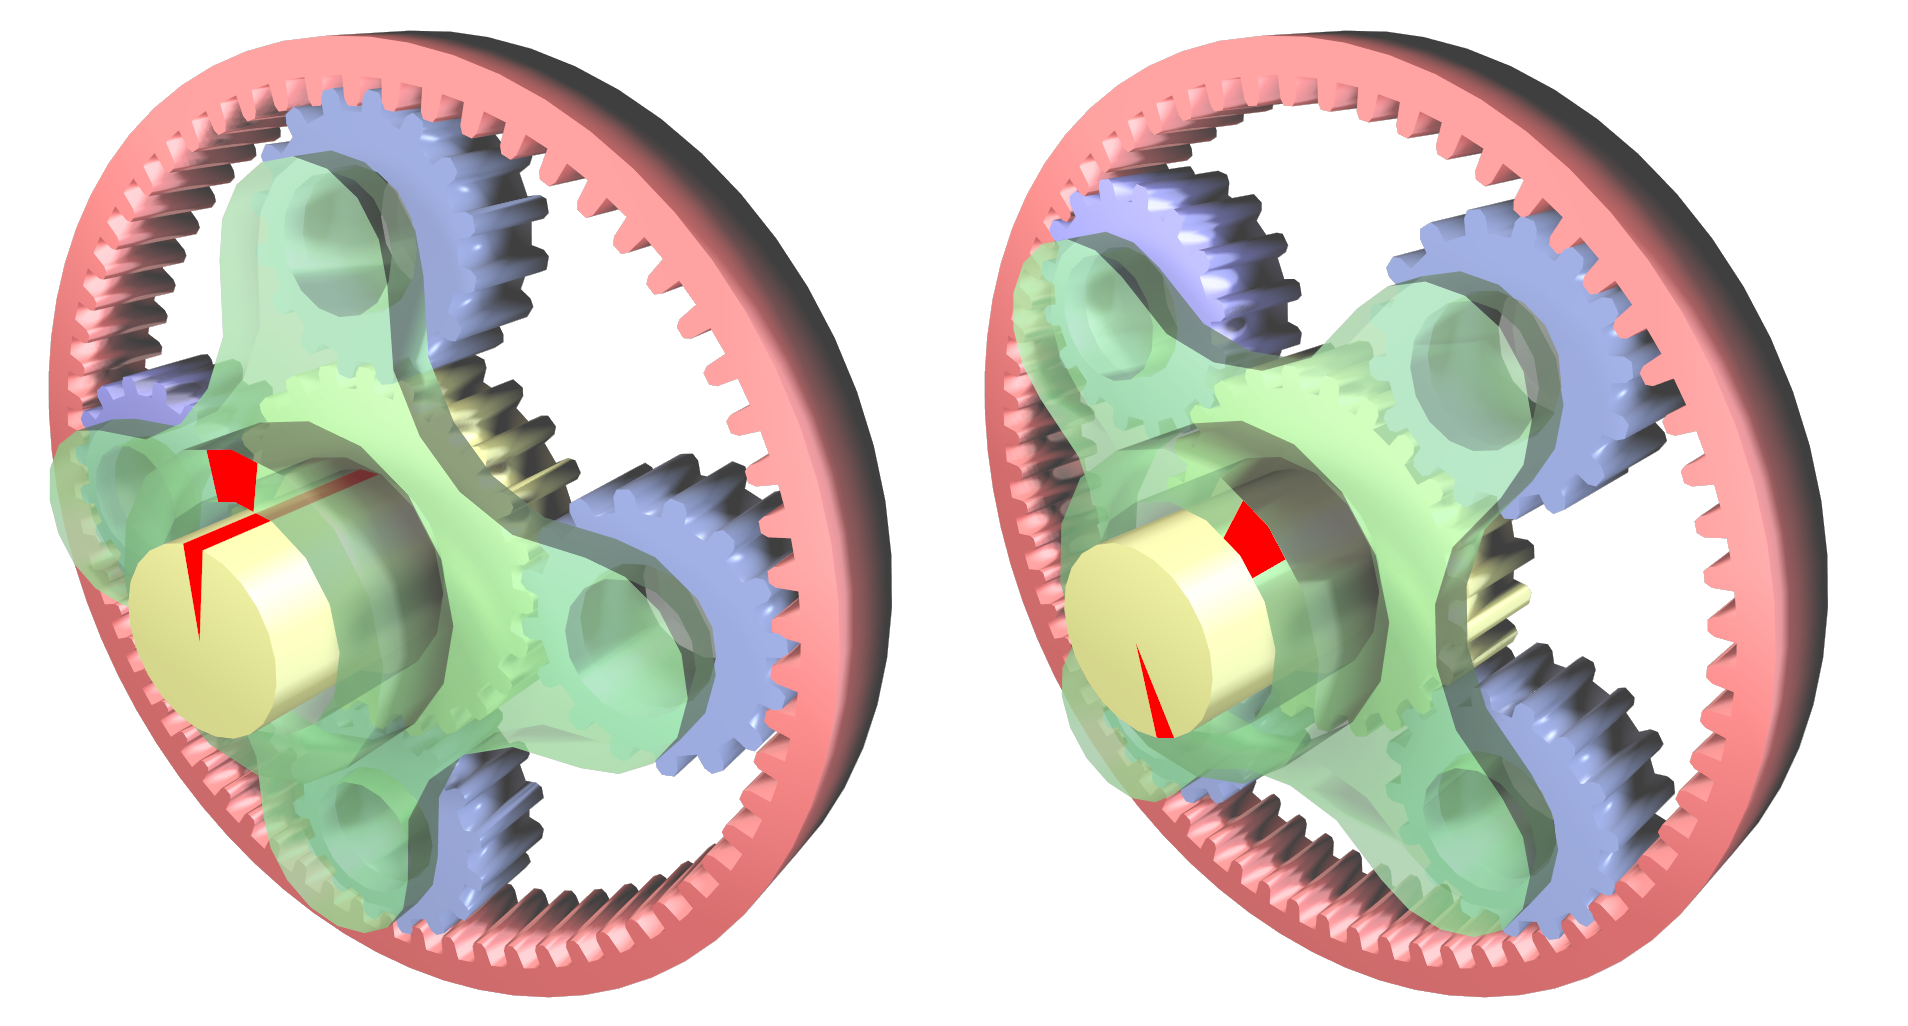
\includegraphics[width = 0.9\textwidth]{epicyclicgear}
						\caption{Planetengetriebe mit Sonnenrad (gelb), Planetenrädern (blau), Planetenradträger (grün) sowie Hohlrad (rot). Das rechte Bild zeigt die relative Verschiebung von Sonnenrad und Planetenradträger, nachdem letzterer um \ang{45} rotiert wurde. Quelle:~\url{https://commons.wikimedia.org/wiki/File:Epicyclic_gear_ratios.png}}
					\end{figure}
				% end

				\subsubsection{Harmonic Drive Getriebe}
					Ein \emph{Harmonic Drive Getriebe} besteht aus:
					\begin{itemize}
						\item Elliptischer \emph{Wave Generator} \\ Elliptische Stahlscheibe mit zentrischer Nabe sowie aufgezogenem elliptisch Verformbaren Kugellager.
						\item \emph{Flexspline} \\ Zylindrische, verformbare Stahlbüchse mit Außenverzahnung.
						\item \emph{Circular Spline} \\ Zylindrischer Ring mit Innenverzahnung.
					\end{itemize}
				
					Dabei wir der elliptische Wave Generator angetrieben und verformt über das Kugellager den Flexspline. Dieser befinet sich gegenüber der großen Ellipsenachse mit dem Circular Spline im Eingriff. Drehen des Wave Generators führt zu einer Verlagerung der großen Ellipsenachse und damit zu einer Verlagerung  des Zahneingriffsbereichs von Flexspline und Circular Spline. Eine halbe Umdrehung des Wave Generators führt dann zu einer Relativbewegung zwischen Flexspline und Circular Spline um einen Zahn.
					
					\begin{itemize}
						\item \textbf{Vorteile:}
							\begin{itemize}
								\item Spielfreiheit (\dh es existiert kein Spiel).
								\item Sehr genaue Positionier- und Wiederholgenauigkeit
								\item Kompakte Bauweise.
								\item Hohe Drehmomentkapazität.
								\item Hoher Wirkungsgrad.
								\item Hohe Torsionssteifigkeit (\dh das Getriebe ist sehr resistent gegenüber Verformungen).
								\item Hohe Zuverlässigkeit und lange Lebensdauer.
							\end{itemize}
						\item \textbf{Nachteile:}
							\begin{itemize}
								\item Teuer.
								\item War bislang nicht beliebig klein realisierbar, neue Entwicklungen ermöglichen aber auch kleine Varianten.
							\end{itemize}
					\end{itemize}
				% end
			% end
		% end

		\section{Alternative und elastische Antriebskonzepte} % 6.30, 6.31, 6.32
			\todo{Content}

			\subsection{Beine} % 6.33, 6.34
				\todo{Content}
			% end

			\subsection{Neue Materialien} % 6.35, 6.36, 6.36, 6.37, 6.42
				\todo{Content}
			% end

			\subsection{Compliant Robot Actuation} % 6.38
				\todo{Content}
			% end

			\subsection{Elastische Antriebskonzepte} % 6.45
				Die Grundidee ist die Kombination elektrischer Antriebe mit mechanischer (potentiell verstellbarer) Elastizität.
				
				\begin{itemize}
					\item Seriell-Elastische Antriebe (SEA):
						\begin{itemize}
							\item \textbf{Stärken:}
								\begin{itemize}
									\item Energiespeicherung reduziert die benötigte Leistungsspitze des Motors und den Energieverbrauch.
									\item Die Entkopplung von Antrieb und Abtrieb liefert Stoßkompensation.
									\item Sicherheitspotential.
								\end{itemize}
							\item \textbf{Schwächen:}
								\begin{itemize}
									\item Erhöhte Masse des Antriebssystems.
									\item Erhöhte Komplexität der mechanischen Konstruktion.
									\item Erhöhte Komplexität der Regelung.
								\end{itemize}
						\end{itemize}
					\item Parallel-Elastische Antriebe (PAE):
						\begin{itemize}
							\item \textbf{Stärken:}
								\begin{itemize}
									\item Energiespeicherung reduziert die benötigte Leistungsspitze des Motors und den Energieverbrauch, allerdings potentiell auch das Motordrehmoment bei SPitzen.
								\end{itemize}
							\item \textbf{Schwächen:}
								\begin{itemize}
									\item Erhöhte Masse des Antriebssystems.
									\item Erhöhte Komplexität der mechanischen Konstruktion.
									\item Erhöhte Komplexität der Regelung.
								\end{itemize}
						\end{itemize}
				\end{itemize}

				\subsubsection{Variable Stiffness Actuator} % 6.46
					\todo{Content}
				% end

				\subsubsection{Variable Impedance Actuators} % 6.47, 6.48, 6.49, 6.50, 6.51
					\todo{Content}
				% end
			% end

			\subsection{Vom Muskel-Skelett-Apparat inspirierte Roboter} % 6.52, 6.53
				\todo{Content}
			% end
		% end
	% end

	\chapter{Sensoren}
		Ein \emph{Sensor} ist ein technisches System, welches eine physikalische (analoge) Größe (\zB Position) und gegebenenfalls deren Änderung (\zB Geschwindigkeit) in geeignete (unsicherheitsbehaftete) elektronische (digitale) Signale transformiert.
		
		Ein \emph{internen Sensor} ("proprioceptive sensor") erfasst dabei die Roboter-internen Zustände, wobei ein \emph{externer Sensor} ("exteroceptive sensor") Informationen über den Zustand der Umwelt sammelt.
	
		\section{Interne Sensoren}
			Interne Sensoren können grob in die Kategorien
			\begin{itemize}
				\item Positionssensoren
				\item Geschwindigkeitssensoren
				\item Beschleunigungssensoren
				\item Inertial Navigation System (INS)
				\item Kraft-Momenten-Sensoren
			\end{itemize}
			unterteilt werden.

			\subsection{Positionssensoren}
				\subsubsection{Potentiometer}
					Ein \emph{Potentiometer} besteht aus einem \emph{Widerstandselement} mit darüber verlaufender Spannung und einem gleitendem Kontakt (\emph{Wischer}, "wiper"), der sich Über das Widerstandselement bewegt. Dabei kann sich entweder der Wischer oder das Widerstandselement bewegen. Abbildung~\ref{fig:potentiometer} zeigt ein lineares und ein rotatorisches Potentiometer.
					
					Die Spannung im Kontakt ist dann abhängig von der Position auf dem Widerstandselement und damit proportional zur Gelenkposition, womit die Position gemessen werden kann. Die Genauigkeit liegt (unter der Voraussetzung einer stabilen Spannungsquelle) bei ca. \SI{0.5}{\percent}.
					
					\begin{figure}
						\centering
						\begin{tikzpicture}
							\node [minimum width = 0.8cm] (a) {+\si{\volt}};
							\node [minimum width = 0.8cm, below = 2 of a] (b) {\SI{0}{\volt}};
							
							\draw [fill = tud2b, color = tud2b] (a.south east) -- (b.north east) -- (b.north west) -- (a.south west) -- cycle;
							
							\path (a.east) to coordinate(c) (b.east);
							\node [right = 1.6 of c] (A) {\(\si{\volt}_\text{aus}\)};
							\coordinate [right = 0.1 of c] (B);
							\draw [->, color = tud7b, line width = 4pt, > = { Latex[length = 4mm] }] (A) -- (B);
						\end{tikzpicture}
						\hspace{1cm}
						\begin{tikzpicture}[xscale = 0.8, yscale = 0.8]
							\node at (0.65, 0.1) {+\si{\volt}};
							\node at (0.5, -0.9) {\SI{0}{\volt}};
							
							\draw [line width = 0.4cm, color = tud2b] (0, 0) arc (0:340:2cm);
							
							\draw [->, color = tud7b, line width = 4pt, > = { Latex[length = 4mm] }] (-2cm, 0) to node[above, color = black, yshift = -1pt]{\(\si{\volt}_\text{aus}\)} (-0.3cm, 0);
							
							\draw [fill = black] (-2cm, 0) circle (0.15cm);
						\end{tikzpicture}
						\caption{Lineares (links) und rotatorisches (rechts) Potentiometer mit Widerstandselement (blau) und Kontakt (orange).}
						\label{fig:potentiometer}
					\end{figure}
				% end

				\subsubsection{Optische Codierer}
					Auf einer Scheibe wird ein kodiertes Muster angebracht, welches den Strahl einer Lichtquelle periodisch unterbricht, wobei diese Quelle auf einen Photodetektor ausgerichtet ist. Durch Messung der Unterbrechung kann die Position gemessen werden. Dabei werden zwei Arten von optischen Kodierern unterschieden:
					\begin{itemize}
						\item Inkrementelle Codierer
						\item Absolute Codierer
					\end{itemize}

					\paragraph{Inkrementell}
						Die Empfangseinheit zählt die Inkremente (die durch die periodischen Unterbrechungen erzeugt werden) und zählt diese (daher der Name \emph{inkrementeller Codierer}). Daraus kann anschließend die Position berechnet werden. Einer großer Nachteil dieser Methode ist, dass die Startposition unbekannt ist, \dh der Zähler muss zunächst Kalibriert werden.
						
						Durch mehrspurige Codierer können durch die Verschiebung der Inkremente mehr Daten gemessen werden:
						\begin{itemize}
							\item 1-spuriger Codierer: Winkel
							\item 2-spuriger Codierer: Winkel und Richtung
							\item 3-spuriger Codierer: Winkel, Richtung, Anfang/Ende
						\end{itemize}
					% end

					\paragraph{Absolut}
						Im Gegensatz zum inkrementellen wird beim \emph{absoluten Codierer} jeder Achsenposition ein individuelles Wortmuster zugeteilt, welches anschließend gemessen wird. Dadurch ist ein direktes Ablesen der Gelenkposition möglich und somit keine Kalibrierung notwendig. Allerdings ist die Konstruktion sehr aufwendig.
						
						Mit dem Gray-Code unterscheidet sich der Code an jeder Stelle nur um ein Bit, wodurch große Fehler vermieden werden.
					% end
				% end

				\subsubsection{Resolver} % 6.63
					\todo{Content}
					
					Resolver sind robust, störungssicher und haben eine hohe Lebensdauer, weshalb sie oft bei Industrierobotern eingesetzt werden.
				% end
			% end

			\subsection{Geschwindigkeitssensoren}
				Geschwindigkeitssensoren lassen sich \bspw durch Differentiation und Filterung aus mit hoher Frequenz abgetasteten Positionswerten erstellen (\dh die Geschwindigkeit wird indirekt gemessen).
			% end

			\subsection{Beschleunigungssensoren (Silizium-Beschleunigungssensor)}
				In einem \emph{Silizium-Beschleunigungssensor} befindet sich eine träge Masse in einem "Siliziumbad", wobei Auslenkungen der Aufhängung die mechanischen Spannungen ändern, wodurch der piezoresistive Widerstandswert geändert wird. Dieser Wert ist messtechnisch erfassbar, wodurch Beschleunigungen erkannt werden können. Allerdings ist eine Erfassung von Richtung und Betrag der Gravitation nötig, um diese herausrechnen zu können. Durch die Verwendung von drei 1D-Sensoren lässt sich ein 3D-Beschleunigungssensor konstruieren (indem diese orthogonal zueinander angebracht werden).
			% end

			\subsection{Inertial Navigation System (INS)} % 6.67, 6.71
				Die Aufgabe eines \emph{Inertial Navigation Systems} (INS) ist die Bestimmung der Orientierung relativ zu einem Inertialsystem. Dazu lassen sich \bspw folgende Sensoren einsetzen:
				\begin{itemize}
					\item Kompass
					\item Lagesensor
						\begin{itemize}
							\item Hierbei wird eine elektrisch leitfähige Flüssigkeit in einem versiegeltem Glas mit drei Elektronen platziert.
							\item Eine Lageänderung verursacht eine ungleiche Flüssigkeitsverteilung und damit ungleiche Widerstände relativ zum Winkel.
							\item Daraus kann anschließend die Position berechnet werden.
						\end{itemize}
					\item Gyroskop (mechanisch oder mikromechanisch)
				\end{itemize}

				\subsubsection{Mechanisches Gyroskop}
					Ein \emph{Gyroskop} ist ein schnell rotierender, semi-kardanisch aufgehängter Kreisel. Durch die Erdrotation wird ein Drehmoment in Richtung des Medians verursacht, wodurch eine Richtungsanzeige möglich wird.
					
					Angewendet werden Gyroskope an vielen Stellen:
					\begin{itemize}
						\item Linienflugzeug (ca. \num{12} Gyroskope)
						\item Raumstation MIR (\num{11} Gyroskope zur Orientierungshaltung zur Sonne)
						\item Häufig werden 3D-Beschleunigungssensoren für die lineare Beschleunigung und Gyroskope für die 3D-Winkelgeschwindigkeiten verwendet. Die Integration über die Geschwindigkeiten ergibt die zurückgelegte Bewegung (\emph{Odometrie}). Durch Filtern der Messwerte können Fehler und Drifts kompensiert werden.
						\item Ein normales Flugzeug-Gyroskop hat pro Betriebsstunde einen Drift von ca. \SI{1.85}{\kilo\meter}, "High-End"-Gyroskope kommen auf einen Drift von weniger als \SI{0.1}{\percent} der zurückgelegten Distanz.
					\end{itemize}
				% end

				\subsubsection{Mikromechanische Gyroskope}
					Bei mikromechanischen Gyroskopen wird die Rotation durch schwingende, mechanische Elemente registriert. Sie werden \zB als "Stimmgabel" realisiert:
					\begin{itemize}
						\item Zwei Zinken mit unterschiedlichen, festen Schwingfrequenzen.
						\item Bei einer Rotation verursacht die Corioliskraft eine differentielle, sinusförmige Kraft orthogonal zur Hauptschwingung in jedem Zinken.
						\item Durch die differentielle Verbiegungen der Zinken oder die Torsionsschwingung am Stamm der Stimmgabel kann diese Kraft detektiert werden.
						\item Die Anregung der Resonanzfrequenz der Zinken kann elektrostatisch, elektromagnetisch oder piezoresistiv erfolgen
						\item Die durch die Corioliskraft verursachten Schwingungen können kapazitiv, piezoresistiv oder piezoelektrisch detektiert werden.
						\item Eine optische Detektion ist auch möglich, ist \iA allerdings sehr teuer.
					\end{itemize}
				% end
			% end

			\subsection{Kraft-Momenten-Sensoren}
				Zeil von \emph{Kraft-Momenten-Sensoren} ist die Messung der Kräfte und Momente zwischen Effektor und Objekt. Oft wird hierfür eine sogenannte \emph{Kraftmessdose} verwendet, die eine Kombination aus mehreren Messapparaturen darstellt. Typische Apparaturen sind hierbei:
				\begin{itemize}
					\item Dehnungsmessstreifen (DMS)
					\item Piezokristalle
					\item Optische Effekte
				\end{itemize}
				Die Dose wird dabei zwischen Effektor und Roboterhand und -fuß angebracht.
				
				Oft haben Kraft-Momenten-Sensoren eine Speichenradform, wobei auf den Speichen/Stegen Dehnungsmessstreifen angebracht sind. Wirkt eine Kraft auf die Dose, so ändert sich die Länge er Stege. Auf den Dehnungsmessstreifen ist eine dünne Metallfolie in Matrixform angebracht, die bei Änderung der Länge ihren Widerstand ändert. Durch Messung dieser Änderung kann die Krafteinwirkung gemessen werden.
			% end
		% end

		\section{Externe und intelligente Sensoren}
			Abbildung~\ref{fig:sensorsystem_structure} zeigt die typische Struktur eines (externen) Sensorsystems.
			
			\begin{figure}
				\centering
				\begin{tikzpicture}[->, every node/.style = { minimum width = 6cm, minimum height = 0.8cm, draw, rectangle }]
					\node [fill = tud2a] (a) {Umwelt};
					\node [fill = tud8a, below = 0.5 of a] (b) {Sensortechnologie};
					\node [fill = tud8a, below = 0.5 of b] (c) {Aufbereitung/Vorverarbeitung};
					\node [fill = tud8a, below = 0.5 of c] (d) {Verarbeitung/Auswertung};
					\node [fill = tud2a, below = 0.5 of d] (e) {Weltmodellierung/Steuerung/\dots};
					
					\draw (a) -- (b);
					\draw (b) -- (c);
					\draw (c) -- (d);
					\draw (d) -- (e);
				\end{tikzpicture}
				\caption{Typische Struktur eines Sensorsystems, wobei die blau hinterlegten Schritte (größtenteils) analog und die orange hinterlegten Schritte (größtenteils) digital ablaufen.}
				\label{fig:sensorsystem_structure}
			\end{figure}
		
			Externe Sensoren können grob in die Kategorien
			\begin{itemize}
				\item Taktile Sensoren
				\item Näherungssensoren
				\item Abstandssensoren
				\item Positionssensoren
				\item Visuelle Sensoren
			\end{itemize}
			unterteilt werden.

			\subsection{Abstandssensoren}
				\emph{Abstandssensoren} messen den Abstand zwischen dem Sensor und einem Gegenstand. Diese Sensoren sind geeignet zur Erfassung von geometrischen Umweltinformation. Außerdem haben sie eine größere Reichweite als Näherungssensoren.
				
				Es werden drei grundlegende Typen von Abstandssensoren unterschieden:
				\begin{itemize}
					\item Optisch (Nutzung von sichtbaren, elektromagnetischen Wellen)
					\item Radar (elektromagnetische Wellen mit sehr kurzen Längen)
					\item Akustisch (mechanische Wellen)
				\end{itemize}

				\subsubsection{Akustische Abstandssensoren}
					\emph{Schall} ist ein an Materie gebundener Energie- und Impulstransport, wobei eine \emph{Schallwelle} die wellenförmige Ausbreitung der periodischen Anregung eines Übertragungsmediums beschreibt. Der hörbare Schall liegt dabei zwischen \SI{16}{\hertz} und \SI{16}{\kilo\hertz}, wobei alles darunter als \emph{Infraschall} und alles darüber als \emph{Ultraschall} bezeichnet wird.
					
					In den 1980er und 1990er sind Ultraschallsensoren die wichtigsten Sensoren zur Erdfassung der Umwelt. Seit Ende der 1990 werden jedoch vermehrt Laserscanner kombiniert mit Farbkameras eingesetzt. Im Nahbereich sind Ultraschallsensoren jedoch auch noch heute nützlich (Kollisionsdetektion, \bzw -vermeidung), sowie in Bereichen wo weder Laserscanner noch Kameras einsetzbar sind (\zB in Gebäuden mit Rauch).

					\paragraph{Ultraschall}
						Die Messung von Abständen mittels Ultraschall heißt \emph{sonar} ("sound navigation and ranging"). In der Natur wird diese Art der Navigation häufig eingesetzt, \zB von Delfinen und Fledermäusen.
						
						Zur Erzeugung von Ultraschall wird eine schwingende Folie eingesetzt, die im Sende-Modus durch die elektrostatische Kraft, ausgelöst von einer geladenen Aluplatte, vibriert. Im Empfangs-Modus bewegt der Klangdruck die Folie, wodurch sich die Kapazität des Kondensators ändern (elektrostatisches Mikrofon).
						
						Im Normalbetrieb sendet ein Sensor \SI{1}{\milli\second} bis \SI{1.2}{\milli\second} langes "Zwitschern" pro \SI{200}{\milli\second}. Dieses Zwitschern wird aufgrund der unterschiedlichen Materialbeschaffenheit und deren unterschiedlichen Reflexionseigenschaften in unterschiedlichen Frequenzen gesendet.
					% end

					\paragraph{Messsituationen}
						\begin{itemize}
							\item Im Idealzustand ist die Achse der Schallkeule orthogonal zu einem flachen Objekt. In diesem Fall wird ein genauer Abstand gemessen.
							\item Befindet sich ein kleines Objekt vor der Wand, so wird der Abstand weiterhin genau gemessen, die Querposition ist jedoch ungenau.
							\item Steht der Sender rotiert zur Wand, so ist der gemessene Abstand vom Rand der Schallkeule zu kurz (Unterschätzung). Die Unsicherheit des Abstands ist eine Funktion des Rotationswinkels und des Keulenöffnungswinkels.
							\item Ist die Rotation größer als der Keulenöffnungswinkel, so ist die Wand unsicherbar.
							\item Eine Kante ist ebenfalls unsichtbar, solange die Ecke nicht ein wenig abgerundet ist.
							\item Mehrfachreflexionen (wie in einer Ecke) bewirkt eine Starke Überschätzung des Abstands.
						\end{itemize}
					% end

					\paragraph{Abhilfe der Schwierigkeiten}
						Bei nur einem Empfänger darf die Umweltszene nur ein Objekt innerhalb der Schallkeule enthalten der reflektierende Objektteil muss orthogonal zur Strahlrichtung stehen.
						
						Gebräuchliche Abhilfen sind die Verwendung von mehreren Ultraschallsensoren und algorithmische Verfahren wie Peilverfahren: Die Position wird aus den Laufzeitunterschieden, \zB mit Triangulationsverfahren (ähnlich wie bei GPS), berechnet.
					% end

					\paragraph{Natur}
						Fledermäuse haben sehr unterschiedliche Ultraschalle (enge Schallkeulen, weite Schallkeulen, Zwitschern mit fester/veränderlicher Frequenz, \dots). Der aktuelle Stand der Ultraschallerzeugung ist vergleichbar mit dem Ultraschall von Fledermäusen, allerdings liegen die technischen Fähigkeiten zur Verarbeitung noch weiter hinter jenen von Fledermäusen.
					% end
				% end

				\subsubsection{Optische Abstandssensoren}
					Der Aufbau von optischen Abstandssensoren besteht aus einem Emitter (LED, Laserdioden) und einem Empfänger (Fototransistor). Optische Sensoren liefern sehr genaue Entfernungsmessungen und sind stabil gegen viele Fremdeinflüsse.
					
					Es gibt verschiedene Messverfahren:
					\begin{itemize}
						\item Ermittlung der Flugzeit (Laufzeit)
						\item aktive Triangulation
						\item Interferometrie (Phasenverschiebung)
						\item Stereoskopie
					\end{itemize}

					\paragraph{Laufzeitermittlung}
						Bei der \emph{Laufzeitermittlung} wird die Hin- und Rücklaufzeit eines Impulses (\zB Lichtimpuls) gemessen. Wurde zwischen Aussenden und Empfangen die Zeit \( \Delta t \) gemessen, so berechnet sich die Entfernund \(d\) wie folgt:
						\begin{equation*}
							d = \frac{c \cdot \Delta t}{2}
						\end{equation*}
						Es muss die Hälfte genommen werden, da der Lichtstrahl zum Objekt hin und zurück verläuft.
						
						Typische Probleme sind die Absorption des Strahls vom Objekt, Wegreflexion (\zB bei einem Spiegel) sowie Mehrfachreflexion (wodurch der Weg verlängert wird).
					% end

					\paragraph{2D-Laserscanner}
						In einem \emph{Laserscanner} wird ein gepulster Laserstrahl, abgelenkt durch einen beweglichen Spiegel, ausgesandt. Durch diesen Drehspiegel wird die Umgebung fächerförmig abgetastet. Trifft der Impuls auf ein Objekt, so wird er reflektiert und die Entfernung kann mittels Laufzeitermittlung berechnet werden. Durch die Abfolge der empfangenen Impulse kann die Entfernung, Lage und Kontur eines Objekts berechnet werden.
						
						Bei der \emph{Kartografierung} werden alle gescannten Szenen (gescannt mit einem mobilen System) zu einer Karte zusammengefasst.
					% end
				% end
			% end

			\subsection{Visuelle Sensoren}
				\begin{itemize}
					\item Visuelle Wahrnehmung ("visual perception")
						\begin{itemize}
							\item Aufnahme und Verarbeitung von visuelle Reizen
							\item Auge und Gehirn extrahieren relevante Informationen
							\item Erkennen von Elementen und deren Interpretation und Abgleich mit Erinnerungen
						\end{itemize}
					\item Maschinelles Sehen ("machine vision")
						\begin{itemize}
							\item Digitale Bildverarbeitung und Mustererkennung
							\item Eingesetzt \zB bei Prüfverfahren in der industriellen Fertigung
						\end{itemize}
					\item Bildverstehen ("computer vision")
						\begin{itemize}
							\item Extraktion komplexer Interpretationen und Schlüsse aus 2D-Abbildungen realer 3D-Szenen
							\item Viele langfristig orientierte Grundlagenforschungsfragen
						\end{itemize}
					\item Robotersehen ("robot vision")
						\begin{itemize}
							\item Maschinelles Sehen und Bildverstehen unter den Echtzeitbedingungen eines Roboters
							\item Begrenze Rechenleistung und schnelle Reaktionszeiten
						\end{itemize}
				\end{itemize}
			
				Voraussetzungen für maschinelles Sehen sind:
				\begin{enumerate}
					\item "Technisches Auge", \dh ein Kamerachip mit Optik
					\item "Intelligente", bildverarbeitende Algorithmen
					\item Ausreichende Strukturierung (Material, Merkmale der relevanten Objekte, \dots) der Szene
					\item Ausreichende Beleuchtung (Helligkeit, Lampen-Lichtspektrum, Reflexionen, \dots) der Szene
				\end{enumerate}
				Je nach Aufgabe ist eine Abstimmung dieser vier Voraussetzungen nötig, \dh es gibt keine allgemeine Lösung.
				
				Die klassische Hierarchie der Bildverarbeitungsoperationen ist in Abbildung~\ref{fig:image_processing_hierarchy} aufgezeigt.
				
				\begin{figure}
					\centering
					\begin{tikzpicture}[block/.style = { draw, rectangle, minimum height = 0.8cm, align = center }, minwidth/.style = { minimum width = 7cm }]
						\node [block, minimum width = 2cm] (a) {Szene};
						\node [block, minwidth, below = 0.5 of a] (b) {\textbf{Bilderzeugung}};
						\node [block, minwidth, below = 0.5 of b] (c) {\textbf{Bildvorverarbeitung} \\ Rauschunterdrückung};
						\node [block, minwidth, below = 0.5 of c] (d) {\textbf{Bildverarbeitung} \\ Segmentierung (Partitionierung)};
						\node [block, minwidth, below = 0.5 of d] (e) {\textbf{Bildbeschreibung} \\ Merkmalsextraktionen: \\ räumlich (Größe, Form) oder spektral};
						\node [block, minwidth, below = 0.5 of e] (f) {\textbf{Objekterkennung}};
						\node [block, minwidth, below = 0.5 of f] (g) {\textbf{Bildanalyse} \\ Interpretation der Szene \\ durch symbolische Beschreibung};
						\coordinate [below = 0.5 of g.south east] (h);
						
						\node [left = 0 of b] {Pixel};
						\node [left = 0 of d] {Kanten};
						\node [left = 0 of e] {Konturen};
						\node [left = 0 of f] {Objekte};
						\node [left = 0 of g] {Semantik};
						
						\path (b.south east) to coordinate(B) (c.north east);
						\path (c.south east) to coordinate(C) (d.north east);
						\path (d.south east) to coordinate(D) (e.north east);
						\path (e.south east) to coordinate(E) (f.north east);
						\path (g.south east) to coordinate(G) (h.north east);
						
						\node [right = 0 of B] {Rohbild (degradiert)};
						\node [right = 0 of C] {Fertigbild (korrigiert)};
						\node [right = 0 of D] {Segmentiertes Bild};
						\node [right = 0 of E] {Merkmale, \ggf auch 3D};
						\node [right = 0 of G] {Relevante Aussage};
						
						\draw [->] (a) -- (b);
						\draw [->] (b) -- (c);
						\draw [->] (c) -- (d);
						\draw [->] (d) -- (e);
						\draw [->] (e) -- (f);
						\draw [->] (f) -- (g);
					\end{tikzpicture}
					\caption{Klassische Hierarchie der Bildverarbeitung. Dabei findet alles bis zur Bildverarbeitung numerisch und alles ab der Bildbeschreibung symbolisch statt.}
					\label{fig:image_processing_hierarchy}
				\end{figure}

				\subsubsection{Bilderzeugung}
					Die \emph{Kameramatrix} beschreibt die Projektionsabbildung von 3D-Punkten durch eine Lochkamera auf 2D-Punkte der Bildebene. Dadurch können spezifische Verzerrungseffekte der Kameralinse berücksichtigt werden.
					
					Zur Bilderzeugung gibt es mehrere grundlegende Methoden von Bildwandlersystemen (Kamerachip):
					\begin{itemize}
						\item Binäre fotoelektrische Zellen \\ Der Chip besteht aus einzelnen Fotodioden, wobei die Bildpunkte entweder \num{1} oder \num{0} wahrnehmen (hell oder dunkel).
						\item Zeilen von Fotodioden (Linearkamera) \\ Die fotoelektrischen Zellen sind entlang einer Geraden angeordnet.
						\item Felder von Fotoelementen (Matrixkamera) \\ Die Zellen sind zweidimensional Angeordnet.
						\item CCD-Fernsehkameras \\ Fernsehnorm, vorgeschaltete Kameraoptik, \dots
					\end{itemize}
				% end

				\subsubsection{Grundlagen}
					Die \emph{Lichtintensitätsfunktion} \( f^\ast \), die für einen Pixel \( (x, y) \) die Lichtintensität \( [f^\ast] = \si{\candela} \) angibt, kann in ein Produkt
					\begin{equation*}
						f^\ast(x, y) = i(x, y) \cdot r(x, y)
					\end{equation*}
					aufgespalten werden mit der Illuminationsfunktion \( i(x, y) \) und der Reflexionsfunktion \( 0 < r(x, y) < 1 \). Dabei hat die Illuminationsfunktion die Einheit \( [i] = \si{\candela} \) (Candela) und die Reflexion ist einheitenlos. Beispielhafte Werte für die Illumination \(i\) und die Reflexion \(r\) sind in den Tabellen~\ref{tab:example_illumination} und~\ref{tab:example_reflexion} gegeben.
					
					Die Absorptionsfunktion
					\begin{equation*}
						a(x, y) \coloneqq 1 - r(x, y)
					\end{equation*}
					beschreibt, wie viel Licht an einem Pixel \( (x, y) \) absorbiert wird/wurde.
					
					\begin{table}
						\centering
						\begin{tabular}{l|l}
							Ort          & Illumination \(i\)   \\ \hline
							Sonne        & \SI{10000}{\candela} \\
							Wolken       & \SI{1000}{\candela}  \\
							Arbeitsplatz & \SI{100}{\candela}
						\end{tabular}
						\caption{Beispielhafte Werte der Illumination \(i\).}
						\label{tab:example_illumination}
					\end{table}
					\begin{table}
						\centering
						\begin{tabular}{l|l}
							Material       & Reflexion \(r\) \\ \hline
							Schwarzer Samt & \num{0.01}      \\
							Edelstahl      & \num{0.65}      \\
							Weiße Wand     & \num{0.80}      \\
							Spiegel        & \num{0.90}      \\
							Schnee         & \num{0.93}
						\end{tabular}
						\caption{Beispielhafte Werte der Reflexion \(r\).}
						\label{tab:example_reflexion}
					\end{table}
				
					Zusammengefasst ergibt sich die \emph{Bildmatrix} \( f = (f_{i, j}) \)
					\begin{equation*}
						f =
							\begin{bmatrix}
								f_{0, 0}     & f_{0, 1}     & \cdots & f_{0, N - 1}     \\
								\vdots       & \vdots       & \ddots & \vdots           \\
								f_{M - 1, 0} & f_{M - 1, 1} & \cdots & f_{M - 1, N - 1}
							\end{bmatrix}
					\end{equation*}
					mit den Elementen als Werten der Lichtintensitätsfunktion. Typische Formate \( M \times N \) sind
					\begin{itemize}
						\item PAL:  \tabto{1.5cm} \( N = \num{768} \),  \tabto{3.5cm} \( M = \num{576} \)  \tabto{5.5cm} (576i50)
						\item NTSC: \tabto{1.5cm} \( N = \num{640} \),  \tabto{3.5cm} \( M = \num{480} \)  \tabto{5.5cm} (480i60)
						\item HDTV: \tabto{1.5cm} \( N = \num{1280} \), \tabto{3.5cm} \( M = \num{720} \)  \tabto{5.5cm} (720p50, WXGA)
						\item HDTV: \tabto{1.5cm} \( N = \num{1920} \), \tabto{3.5cm} \( M = \num{1080} \) \tabto{5.5cm} (1080i50, Full HD)
					\end{itemize}
					Bei einer monochromen Kamera wird pro Bild eine Matrix verwendet, bei einer polychromen Kamera drei Matrizen. Für diese drei Matrizen können unterschiedliche Farbmodelle verwendet werden, z.\,B.:
					\begin{itemize}
						\item RGB (Red, Green, Blue) \\ Speziell für Monitore relevant, da diese meistens die drei Farben Rot, Grün und Blau anzeigen können.
						\item HSI/HSV (Hue, Saturation, Intensity/Value) \\ Speziell für die Bildverarbeitung, da Segmentierung leicht ist.
					\end{itemize}
					Das RGB-Farbmodell mit \num{8} Bit je Farbe hat damit \( \num{256} \cdot \num{256} \cdot \num{256} = \num{16777216}\text{ mögliche Farben} \).
					
					Eine alternative zum RGB-Modell ist das HSI/HSV-Modell, welches aus den Komponenten
					\begin{itemize}
						\item Hue (Farbwellenlänge)
						\item Saturation (Sättigung, Reinheit der Farbe)
						\item Intensity/Value (Intensität, Helligkeit)
					\end{itemize}
					besteht. Das RGB-Modell mit den Anteilen \(R\), \(G\) und \(B\) lässt sich wie folgt in das HSI/HSV-Modell umrechnen:
					\begin{align*}
						\cos H & = \frac{2R - G - B}{2\sqrt{(R - G)^2 + (R - B)(G - B)}} \\
						S      & = 1 - \frac{3}{R + G + B} \min \{\, R, G, B \,\}        \\
						V = I  & = \frac{1}{3} (R + G + B)
					\end{align*}
					Ein Vorteil des HSI/HSV-Modells ist, dass die Farbmanipulation sehr ähnlich zur menschlichen Wahrnehmung ist.
				% end

				\subsubsection{Bildvorverarbeitung}
					Es gibt zwei Klassen von \emph{Bildvorverarbeitungsverfahren}:
					\begin{enumerate}
						\item \emph{Ortsbereichsverfahren}
							\begin{itemize}
								\item Die Manipulation findet direkt auf der Pixelebene statt.
								\item Die allgemeine Berechnungsformel lautet \( \vec{g}(x, y) = \vec{h}\big(\vec{f}(x, y)\big) \), wobei \(\vec{g}\) die neuen und \(\vec{f}\) die alten Bildintensitäten darstellt. \(\vec{h}\) ist ein Operator, der die Intensität transformiert (\bspw durch Nachbarschaftsbeziehungen).
								\item Aufgrund der geringen Rechenzeit vor allem für Roboter relevant (aufgrund der Echtzeitanforderungen).
							\end{itemize}
						\item \emph{Frequenzbereichsverfahren}
							\begin{itemize}
								\item Es wird zunächst eine Bildtransformation (diskrete Fouriertransformation, Wavelets, \dots) in den Frequenzraum durchgeführt.
								\item Anschließend wird ein Verfahren im Frequenzraum angewandt und das Bild anschließend zurück transformiert.
								\item Wird \bspw bei der Offline-Auswertung von Satellitenbildern eingesetzt.
								\item Aufgrund der hohen Rechenzeit werden diese Verfahren in der Robotik selten eingesetzt.
							\end{itemize}
					\end{enumerate}

					\paragraph{Nachbarschaftsbildverarbeitung}
						Mit der \( n \times n \)-Nachbarschaft eines Pixels \( (x, y) \) wird die Matrix (\bzw die Pixel)
						\begin{equation*}
							\begin{bmatrix}
								(x - \lfloor n/2 \rfloor, y - \lfloor n/2 \rfloor) & \cdots & (x - \lfloor n/2 \rfloor, y) & \cdots & (x - \lfloor n/2 \rfloor, y + \lfloor n/2 \rfloor) \\
								\vdots                                             & \ddots & \vdots                       & \ddots & \vdots                                             \\
								(x, y - \lfloor n/2 \rfloor)                       & \cdots & (x, y)                       & \cdots & (x, y + \lfloor n/2 \rfloor)                       \\
								\vdots                                             & \ddots & \vdots                       & \ddots & \vdots                                             \\
								(x + \lfloor n/2 \rfloor, y - \lfloor n/2 \rfloor) & \cdots & (x - \lfloor n/2 \rfloor, y) & \cdots & (x + \lfloor n/2 \rfloor, y + \lfloor n/2 \rfloor)
							\end{bmatrix}
						\end{equation*}
						bezeichnet, wobei die \(y\)-Achse von links nach rechts und die \(x\)-Achse von oben nach unten wächst. Dies ergibt beispielhaft für die \( 3 \times 3 \)-Nachbarschaft von \( (x, y) \):
						\begin{equation*}
							\begin{bmatrix}
								(x - 1, y - 1) & (x - 1, y) & (x - 1, y + 1) \\
								(x, y - 1)     & (x, y)     & (x, y + 1)     \\
								(x + 1, y - 1) & (x + 1, y) & (x + 1, y + 1)
							\end{bmatrix}
						\end{equation*}
						
						In der \emph{Nachbarschaftsbildverarbeitung} wird nun ein solcher Bildausschnitt bezüglich eines Pixels \( (x, y) \) betrachtet und \zB mittels \emph{Nachbarschaftsdurchschnittsbildung} eine neue Intensität des Pixels berechnet. Der folgende Teil beschränkt sich auf \( 3 \times 3 \)-Nachbarschaften, theoretisch sind alle Verfahren aber auch mit größeren Nachbarschaften möglich.
						
						Bei der Nachbarschaftsdurchschnittsbildung wird jeder Pixels eines Bildausschnitts
						\begin{equation*}
							\begin{bmatrix}
								f_1 & f_2 & f_3 \\
								f_4 & f_5 & f_6 \\
								f_7 & f_8 & f_9
							\end{bmatrix}
						\end{equation*}
						mit einem Gewicht \( \omega_1, \cdots, \omega_9 \) (wobei \( \sum_{k = 1}^{9} \omega_k = 1 \) gelten muss) multipliziert, was sogenannte \emph{Gewichtsmaske} darstellt. Diese wird häufig auch durch eine Matrix
						\begin{equation*}
							\mat{\omega} =
								\begin{bmatrix}
									\omega_1 & \omega_2 & \omega_3 \\
									\omega_4 & \omega_5 & \omega_6 \\
									\omega_7 & \omega_8 & \omega_9
								\end{bmatrix}
						\end{equation*}
						dargestellt. Die neue Intensität \( g_5 \) des zentralen Pixels wird dann durch
						\begin{equation*}
							g_5 = \sum_{k = 1}^{9} \omega_k f_k
						\end{equation*}
						oder Allgemein
						\begin{equation*}
							g = \sum_{k = 1}^{n^2} \omega_k f_k
						\end{equation*}
						berechnet.
						
						Beispiele für Nachbarschaftsfilter:
						\begin{itemize}
							\item Mittelwertbildung:
						\end{itemize}
						\begin{equation*}
							\mat{\omega} =
								\begin{bmatrix}
									1/9 & 1/9 & 1/9 \\
									1/9 & 1/9 & 1/9 \\
									1/9 & 1/9 & 1/9
								\end{bmatrix}
						\end{equation*}
						\begin{itemize}
							\item Detektion isolierter Ausreißer (\zB bei konstant weißem Hintergrund):
						\end{itemize}
						\begin{equation*}
							\mat{\omega} =
								\begin{bmatrix}
									-1 & -1 & -1 \\
									-1 &  8 & -1 \\
									-1 & -1 & -1
								\end{bmatrix}
						\end{equation*}
						
						Ein prinzipielles Problem bei Nachbarschaftsdurchschnittsbildung ist, dass scharfe Bilddetails (\zB Ecken und Kanten) unscharf werden. Eine Abhilfe ist, einen \emph{Median-Filter} zu verwenden. Dabei berechnet sich die neue Intensität \(g\) eines Pixels durch den Medianwert der Intensitäten der Nachbarschaft, \dh ist Intensitäten werden sortiert und es wird der mittlere Wert (der Median) als neue Intensität genutzt.
					% end
				% end

				\subsubsection{Bildverarbeitung}
					Die zentralen Bildverarbeitungsschritte sind \emph{Kantendetektion} (als Voraussetzung für viele Objekterkennungsalgorithmen) und \emph{Segmentierung} (die Zerlegung des Bildes in Komponenten ober Objekte). Dabei werden die zentralen Prinzipien der Unstetigkeiten (zur Kanten- und Konturerkennung) sowie Ähnlichkeit (Schwellwertverfahren, Bereichswachstum) verwendet.

					\paragraph{Kantendetektion}
						Bei der \emph{Kantendetektion} wird verwendet, dass starke, lokale Änderungen der Intensitätsfunktion häufig Projektionen von Kanten der Szene sind. Allerdings entsprechen nicht alle Änderungen der Intensität von tatsächlichen Objektbegrenzungen und nicht alle Begrenzungen führen zu einer starken Änderung der Intensität. Das allgemeine Vorgehen bei der Kantendetektion besteht aus zwei Schritten:
						\begin{enumerate}
							\item Extraktion von Kandidaten für Kantenelemente
							\item Kombination der Elemente zu längeren Strukturen
						\end{enumerate}
					
						Die allgemeine Idee ist, die Größe der ersten Ableitung zur Detektion von Kantenelementen und die Größe der zweiten Ableitung zur Interpretation der Lage der Pixel (negative zweite Ableitung \(\to\) Pixel liegt auf der dunklen, positive zweite Ableitung \(\to\) Pixel liegt auf der hellen Seite der Kante).
						
						Der Gradient einer kontinuierlichen Funktion, differenzierbaren Funktion \( f(x, y) \) ist
						\begin{equation*}
							\nabla f(x, y) =
								\begin{bmatrix}
									\frac{\partial f}{\partial x} \\
									\frac{\partial f}{\partial y}
								\end{bmatrix}
						\end{equation*}
						Problem: \( f(x, y) \), \(x\) und \(y\) stammen aus einem diskreten (ganzzahligen) Wertebereich. Daher muss der Gradient durch den Differenzenquotienten angenähert werden. Dabei können entweder die Vorwärtsdifferenzen
						\begin{equation*}
							\frac{\partial f}{\partial x} = \lim\limits_{h \to 0} \frac{f(x + h, y) - f(x, y)}{h} \approx f(x + 1, y) - f(x, y)
						\end{equation*}
						oder die zentrale Differenzen
						\begin{equation*}
							\frac{\partial f}{\partial x} = \lim\limits_{h \to 0} \frac{f(x + h, y) - f(x - h, y)}{2h} \approx \frac{1}{2} \big( f(x + 1, y) - f(x - 1, y) \big)
						\end{equation*}
						verwendet werden (analog für \( \partial f / \partial y \)). Aufgrund des Mittlungseffekts eignen sich die zentralen Differenzen hier mehr.

						\subparagraph{Prewitt-Operator} % 8.58, 8.59, 8.60, 8.61
							Der \emph{Prewitt-Operator} ist Zusammengesetz auf zwei Filtern: Das Prewitt-X Filter und das \emph{Prewitt-Y Filter}. Ersteres findet Kanten über die \(x\)-Achse, letzterer über die \(y\)-Achse. Diskretisiert ergeben sich folgende Gewichtsmasken:
							\begin{gather*}
								\begin{bmatrix}
									-1 & -1 & -1 \\
									0  & 0  & 0  \\
									1  & 1  & 1
								\end{bmatrix} \tag{Prewitt-X Filter} \\
								\begin{bmatrix}
									-1 & 0 & 1 \\
									-1 & 0 & 1 \\
									-1 & 0 & 1
								\end{bmatrix} \tag{Prewitt-Y Filter}
							\end{gather*}
							Daraus ergeben sich die gefilterten Bilder \(p_x\) (Prewitt-X Filter) und \(p_y\) (Prewitt-Y Filter).
							
							Zusammengesetzt ergibt sich der Prewitt-Operator (\bzw das Graustufenbild)
							\begin{equation*}
								M \approx \sqrt{p_x^2 + p_y^2}
							\end{equation*}
						% end

						\subparagraph{Andere Operatoren} % 8.62, 8.63
							Andere Operatoren zur Kantendetektion sind \bspw der Sobel-Operator und das Roberts-Filter. Zusammengefasst lauten diese:
							\begin{itemize}
								\item Prewitt-Operator:
							\end{itemize}
							\begin{equation*}
								M \approx \sqrt{p_x^2 + p_y^2} \quad\quad\quad\quad
								p_x = \begin{bmatrix}
									-1 & -1 & -1 \\
									0  & 0  & 0  \\
									1  & 1  & 1
								\end{bmatrix} \quad\quad\quad\quad
								p_y = \begin{bmatrix}
									-1 & 0 & 1 \\
									-1 & 0 & 1 \\
									-1 & 0 & 1
								\end{bmatrix}
							\end{equation*}
							\begin{itemize}
								\item Sobel-Operator:
							\end{itemize}
							\begin{equation*}
								M \approx \sqrt{p_x^2 + p_y^2} \quad\quad\quad\quad
								p_x = \begin{bmatrix}
									-1 & -2 & -1 \\
									0  & 0  & 0  \\
									1  & 2  & 1
								\end{bmatrix} \quad\quad\quad\quad
								p_y = \begin{bmatrix}
									-1 & 0 & 1 \\
									-2 & 0 & 2 \\
									-1 & 0 & 1
								\end{bmatrix}
							\end{equation*}
							\begin{itemize}
								\item Roberts-Filter:
							\end{itemize}
							\begin{equation*}
								R = \lvert r_x \rvert + \lvert r_y \rvert \quad\quad\quad\quad
								r_x = \begin{bmatrix}
									-1 & 0 \\
									0  & 1
								\end{bmatrix} \quad\quad\quad\quad
								r_y = \begin{bmatrix}
									0 & -1 \\
									1 & 0
								\end{bmatrix}
							\end{equation*}
						% end
					% end

					\paragraph{Konturerkennung}
						\subparagraph{Lokale Analyse}
							Es wird die lokale Nachbarschaft eines Pixels \( (x, y) \) untersucht. Außerdem werden regelbasierte Verbindungen von Kandidaten für Kantenelemente durchgeführt:
							\begin{itemize}
								\item Wenn \( \big\lvert \nabla f(x, y) - \nabla f(\tilde{x}, \tilde{y}) \big\rvert \leq T \), \( T > 0 \) (die Gradienten sind Betragsmäßig ähnlich) \\ und \( \big\lvert \alpha(x, y) - \alpha(\tilde{x}, \tilde{y}) \big\rvert < A \), \( A > 0 \) (die Winkel der Gradientenvektoren sind ähnlich), dann:
								\item Verbinde \( (x, y) \) mit \( (\tilde{x}, \tilde{y}) \) und kennzeichne diese Verbindung (\zB durch einen bestimmten Grauwert/eine bestimme Farbe oder ein Symbol).
							\end{itemize}
							Dabei ist
							\begin{equation*}
								\alpha(x, y) \coloneqq \arctan \frac{\partial f / \partial y}{\partial f / \partial x}
							\end{equation*}
							der Winkel des Gradientenvektors.
						% end

						\subparagraph{Globale Analyse und Hough-Transformation}
							Die globale Analyse geschieht durch eine sogenannte \emph{Hough-Transformation}. Dabei werden mehrere Punkte verbunden, sofern diese auf einer vorgegebenen Kurve (\zB eine Gerade oder eine Parabel) liegen. Im folgende wird Beispielhaft die Hough-Transformation \bzgl einer Geraden betrachtet, prinzipiell kann sie aber für jede durch eine Gleichung
							\begin{equation*}
								g(x, y, c_1, c_2, c_3) = 0
							\end{equation*}
							gegebene Kurve durchgeführt werden (\zB für einen Kreis \( (x - c_1)^2 + (y - c_2)^2 - c_3^2 = 0 \) mit Radius \( c_3 \)).
							
							Liegen Punkte \( (x_i, y_i) \) auf einer Geraden, so erfüllen diese die Gleichung \( y_i = ax_i + b \) mit den Parametern \(a, b\). Diese Gleichung kann mit
							\begin{equation*}
								y_i = ax_i + b \quad\iff\quad b = -x_ia + y_i
							\end{equation*}
							zu einer Geradengleichung im Parameterraum \( (a, b) \) umgeformt werden. Bei der Hough-Transformation wird nun jeder Punkt \( (x_i, y_i) \) einer Geraden in der \( (a, b) \)-Ebene zugeordnet. Liegen zwei Punkte \( (x_i, y_i) \) und \( (x_j, y_j) \) auf einer Geraden, so schneiden sich die Hough-Transformierten in einem Punkt. Dieser Schnittpunkt \( (a^\ast, b^\ast) \) entspricht den Parameter der Geraden, auf der die zwei Punkte liegen, \dh es gilt:
							\begin{equation*}
								y_i = a^\ast x_i + b^\ast \quad\quad\text{und}\quad\quad y_j = a^\ast x_j + b^\ast
							\end{equation*}
							Schneiden sich drei Graden in einem Punkt, so liegen alle entsprechenden Punkte auf einer Geraden.
							
							In der Praxis ist die Darstellung \( y = ax + b \) der Geraden problematisch, da vertikale Geraden nicht dargestellt werden. Es wird daher eher die Parametrisierung \( x \cos\theta + y \sin\theta = \rho \) verwendet, da hier das Problem nicht auftritt.
							
							% TODO: Hough-Transformation: Beispiel.
						% end
					% end

					\paragraph{Segmentierung}
						Ziel der \emph{Segmentierung} ist, das Bild \(B\) ein flächige \emph{Zusammenhangkomponenten} \( S_1, \cdots, S_n \) zu zerlegen, wobei diese paarweise disjunkt sind und \( S_1 \cup \cdots \cup S_n = B \) gilt. Dazu müssen die Grenzen von Objektflächen gefunden werden, die für die weitere Interpretation von Bedeutung sind.

						\subparagraph{Schwellwertabfrage}
							Dieses Verfahren wird häufig verwendet und ist insbesondere im HSI/HSV-Farbraum sehr nützlich. Bezogen auf die Intensität \( f(x, y) \) werden zwei Schwellwerte \( \tau_1, \tau_2 \) festgelegt, wodurch sich über
							\begin{equation*}
								g(x, y) \coloneqq
									\begin{cases*}
										0 & \text{falls } \( f(x, y) < \tau_1 \) \\
										1 & \text{falls } \( \tau_1 < f(x, y) < \tau_2 \) \\
										2 & \text{falls } \( \tau_2 < f(x, y) \)
									\end{cases*}
							\end{equation*}
							ein trinäres Schwellwertbild ergibt.
							
							Dieses Verfahren wirft allerdings Probleme auf, da die Intensitätsfunktion stark von der aktuellen Beleuchtung abhängig ist, welche von Bild zu Bild variieren kann. Eine automatische Adaption der Schwellwerte erfordert eine robuste Minimum-Suche, wobei die Minima abhängig sind von Beleuchtung, Lager der Objekte, \dots.
						% end

						\subparagraph{Bereichswachstum}
							\begin{itemize}
								\item Es wird mit einem oder mehreren geeigneten "Saat"-Punkten ("seed points") gestartet und die direkten Nachbarpixel überprüft.
								\item Ein untersuchter Pixel wird zu dem Bereich des Startpixels hinzugefügt, wenn dieser dem Startpixel ähnlich ist (\zB gleicher Grauwert, Farbe, Textur, \dots).
								\item Unterscheidet sich der Pixel stark, so wird ein neuer Bereich eröffnet.
								\item Anschließend wird das Bild rekursiv weiter untersucht.
								\item Weitere Operationen können \zB das Aufteilen und Verbindungen von Bereichen sein.
							\end{itemize}
						% end
					% end
				% end

				\subsubsection{Merkmalsextraktion}
					Bisher wurden Objekte Bildhaft durch diskrete Bildfunktionen beschrieben. Die \emph{Merkmalsextraktion} beschäftigt sich nun mit der Charakterisierung von Objekten durch einen Vektor von Merkmalen sowie eventuell Beziehungen zwischen Objekten (Relationstupel) wie Nachbarschaft und Größe. Ausgangspunkt ist dabei das durch Segmentierung und Bildvorverarbeitung entstandene Binärbild \( g(x, y) \). Ziel ist die Extraktion der Merkmale, die ein Segment beschreiben.
					
					Merkmale können \zB sein:
					\begin{itemize}
						\item \(m_1\): Objektumfang \( m_1 = \int_\text{Kontur} \! g(x, y) \dif{s} \approx \sum_\text{Kontur} g(x, y) \)
						\item \(m_2\): Objektfläche \( m_2 = \iint \! g(x, y) \dif{x} \dif{y} \approx \sum_x \sum_y g(x, y) \)
						\item \(m_3\): Anzahl der "Löcher"
						\item \(m_4\): Farbe
						\item \dots
					\end{itemize}
					Solche Merkmale sollten möglichst (weitgehend)
					\begin{itemize}
						\item invariant gegen Skalierung, Rotation sowie Translation,
						\item robust (gegen Rauschen), signifikant, diskriminierend (unterscheidbar) sowie
						\item schnell berechenbar sein.
					\end{itemize}
				% end

				\subsubsection{Objektklassifikation}
					\begin{itemize}
						\item Klassische Ansätze zur Objektklassifikation:
							\begin{itemize}
								\item Bildvergleich im Merkmalsraum
								\item Template Matching
							\end{itemize}
						\item In den letzten Jahren wurden große Fortschritte durch Deep Learning erzielt.
						\item Deep Learning Systeme scheitern allerdings noch an einem echten Verstehen der Objekte.
					\end{itemize}
				% end
				
				\subsubsection{Bildverstehen} % 8.87, 8.88, 8.89, 8.90, 8.91, 8.92
					\todo{Content}
				% end
			% end

			\subsection{3D-Sensoren und Perzeption}
				Bei einem einzelnen RGB-Pixel eines 2D-Farbbildes fließen viele Faktoren ein:
				\begin{itemize}
					\item Lichtquelle (Anzahl, Helligkeit, Farbspektrum)
					\item Objekte (Farbe, physikalische Eigenschaften wie Transparenz und Reflexion)
					\item Szene (Schattenwurf)
					\item Projektion (Perspektivische Verzerrung)
					\item Sensorqualität
				\end{itemize}
				Ein Mensch ist extrem gut darin, aus einem einzelnen Bild Tiefeninformationen zu extrahieren, wobei dies im Bereich Computer Vision noch immer eine große Herausforderung ist.
				
				Werden zwei Farbbilder (leicht versetzt) verwendet, so wird dies als \emph{Stereo Vision} (oder in der Biologie auch "binokulares Sehen") bezeichnet. Dies erlaubt eine passive Tiefenschätzung. Andere Spezies wie Fledermäuse haben sogar eine aktive Tiefenschätzung (Sonar).
				
				Distanzinformationen sind extrem wichtig:
				\begin{itemize}
					\item 3D-Navigation
					\item Interaktion
					\item Kollisionsvermeidung
					\item Objekterkennung
					\item Gestenerkennung
					\item Virtual/Augmented Reality
					\item \dots
				\end{itemize}

				\subsubsection{Bildbasierte 3D-Sensoren}
					\paragraph{Stereo Vision}
						\emph{Stereo Vision} basiert auf der Triangulation von Bildpunkten durch die Verwendung von zwei Bildern.
						
						Basierend auf Abbildung~\ref{fig:stereo_triangulation} kann die Distanz \(Z\) wie folgt berechnet werden:
						\begin{equation*}
							\frac{Z - f}{B - (x - x')} = \frac{Z}{B} \quad\iff\quad BZ - Bf = BZ - Z(x - x') \quad\iff\quad Z = \frac{Bf}{x - x'}
						\end{equation*}
						
						\begin{figure}
							\centering
							\begin{tikzpicture}
								\node [fill = black, draw, circle, label = above:{\(X\)}] (X) at (0, 0) {};
								\node [fill = black, draw, circle] (x) at (-3, -6) {};
								\node [fill = black, draw, circle] (xPrime) at (3, -6) {};
								\node [fill = black, draw, circle, label = below:{\(O\)}] (o) at (-4, -8) {};
								\node [fill = black, draw, circle, label = below:{\(O'\)}] (oPrime) at (4, -8) {};
								
								\path let \p1 = (o), \p2 = (x) in coordinate (f) at (\x1, \y2);
								\path let \p1 = (oPrime), \p2 = (xPrime) in coordinate (fPrime) at (\x1, \y2);

								\coordinate [above = 0.1 of x] (xShift);
								\coordinate [above = 0.1 of xPrime] (xPrimeShift);
								
								\path let \p1 = (xShift), \p2 = (f) in coordinate (fShift) at (\x2, \y1);
								\path let \p1 = (xPrimeShift), \p2 = (fPrime) in coordinate (fPrimeShift) at (\x2, \y1);
								
								\coordinate [left = 2 of x] (xShiftLeft);
								\coordinate [right = 0.2 of x] (xShiftRight);
								\coordinate [left = 0.2 of xPrime] (xPrimeShiftLeft);
								\coordinate [right = 2 of xPrime] (xPrimeShiftRight);
								
								\path (o) to coordinate(oCenter) (oPrime);
								
								\draw (o) to node[below]{Baseline \(B\)} (oPrime);
								\draw [->] (o) to node[left]{\(f\)} (f);
								\draw [->] (oPrime) to node[left]{\(f\)} (fPrime);
								\draw [->] (fShift) to node[above]{\(x\)} (xShift);
								\draw [->] (fPrimeShift) to node[above]{\(x'\)} (xPrimeShift);
								\draw (xShiftLeft) to (xShiftRight);
								\draw (xPrimeShiftRight) to (xPrimeShiftLeft);
								\draw (o) to (X);
								\draw (oPrime) to (X);
								\draw [->] (oCenter) to node[right]{\(Z\)} (X);
							\end{tikzpicture}
							\caption{Triangulation der Distanz \(Z\) eines Objekts \(X\) durch zwei Kameras \(O\) und \(O'\).}
							\label{fig:stereo_triangulation}
						\end{figure}
					
						Diese Art der Berechnung wirft das Problem auf, dass detektiert werden muss, welche Pixel das selbe Objekt abbilden.
						
						\begin{itemize}
							\item \textbf{Vorteile:}
								\begin{itemize}
									\item Nur zwei Kameras nötig.
									\item Entspricht dem menschlichen Vorbild (binokulares Sehen).
									\item Farbinformationen sind für jeden Punkt verfügbar.
									\item Hohe Bildraten möglich.
								\end{itemize}
							\item \textbf{Nachteile:}
								\begin{itemize}
									\item Benötigt komplizierte Algorithmen, um die Pixel zuzuordnen.
									\item Erfordert viel CPU Leistung.
									\item Angewiesen auf texturierte Oberflächen (zur Pixelzuordnung).
									\item Sensitiv gegenüber Hintergrundbeleuchtung.
								\end{itemize}
						\end{itemize}
					% end

					\paragraph{Structured Light Kamera} % 8.107, 8.108, 8.109, 8.110, 8.111, 8.112, 8.113, 8.114
						\todo{Content}
					% end

					\paragraph{Stereo Vision + Structured Light} % 8.115, 8.116, 8.117
						\todo{Content}
					% end

					\paragraph{Time-of-Flight (ToF) Kamera}
						Eine \emph{Time-of-Flight} (ToF) Kamera sendet Lichtimpulse (meist Infrarot) und misst die Reflexionen. Hierzu gibt es drei grundlegende Techniken:
						\begin{itemize}
							\item Direct Time-of-Flight Imagers/Flash Lidar
								\begin{itemize}
									\item Direkte Zeitmessung der Lichtstrecke
									\item Benötigt starke Signalflanken (\zB Laserdioden)
								\end{itemize}
							\item Carrier Wave Modulation (Phasenvergleichsverfahren)
								\begin{itemize}
									\item Es wird die Phasenverschiebung des reflektierten Lichtsignals gemessen.
								\end{itemize}
							\item Ranged Gated Imagers ("Shutter")
								\begin{itemize}
									\item Er Shutter öffnet sich in der gleichen Frequenz, in der die Lichtimpulse ausgesendet werden.
									\item Ein reflektierter Impuls wird teilweise vom Shutter blockiert, was einen Rückschluss auf die zurückgelegte Lichtstrecke zulässt.
								\end{itemize}
						\end{itemize}
					
						\begin{itemize}
							\item \textbf{Vorteile:}
								\begin{itemize}
									\item Hohe Bildrate (bis zu \num{160} FPS üblich), daher geeignet für Echtzeitanwendungen
									\item Sehr wenig CPU Leistung nötig.
									\item Musterunabhängig, \dh es werden keine strukturierten/texturierten Oberflächen benötigt.
								\end{itemize}
							\item \textbf{Nachteile:}
								\begin{itemize}
									\item Geringe Auflösung, es sind nur große Pixel realisierbar.
									\item Sensitiv gegenüber Hintergrundbeleuchtung.
									\item Interferenzen zwischen mehreren ToF Kameras.
									\item Mehrfachreflexionen durch großflächige Bestrahlung von Oberflächen.
								\end{itemize}
						\end{itemize}
					% end
				% end

				\subsubsection{Laserbasierte 3D-Sensoren}
					Es ist auch möglich, Tiefeninformationen ohne Kamerabilder zu generieren. Ein Beispiel hierfür sind Laserscanner. Diese können aus mehreren Lasern (Mehrfach-Lasersysteme) zusammengesetzt sein oder dreh-/schwenkbar sein (Mono-Lasersystem). Es ist ebenfalls möglich, Laserscanner und Kamerabilder zu kombinieren, um ein detaillierteres Weltbild zu erhalten.
				% end

				\subsubsection{Datenstrukturen und -Repräsentation}
					Eine klassische, unkomprimierte Punktwolke ("point cloud") benötigt sehr viel Speicherplatz, \dh es werden effektiver Datenrepräsentationen/-strukturen benötigt:
					\begin{itemize}
						\item Reduktion des Speicherbedarfs.
						\item Reduktion des Rechenaufwands bei der Verarbeitung.
						\item Effiziente Aggregation von 3D-Punkten.
						\item Effizienter Zugriff auf einzelne Punkte (\zB Nachbarschaftsinformationen).
					\end{itemize}

					\paragraph{KD-Baum}
						Ein \emph{KD-Baum} ist eine verallgemeinerte Version eines Binärbaums (KD steht für \(k\)-dimensional). Die geometrische Idee ist eine rekursive Aufteilung der Daten mit Hyperebenen.
						
						\begin{itemize}
							\item \textbf{Vorteile:}
								\begin{itemize}
									\item Anwendung der "Branch-and-Bound" Methode: Die Lage des Suchpunktes relativ zum aktuell betrachteten Knoten des Baums verrät, in welchem Unterteilbaum ein potentiell besserer (näherer) Knoten liegt.
									\item Es gibt Algorithmen, die \( \mathcal{O}(\log n) \) garantieren.
									\item Einfach erweiterbar auf \(k\)-nearest Search.
								\end{itemize}
							\item \textbf{Nachteile:}
								\begin{itemize}
									\item Das Einfügen und Entfernen von Punkten ist kompliziert (\ggf Rebalancierung des Baums notwendig).
									\item Keine Datenkompression und Aggregation.
								\end{itemize}
						\end{itemize}
					% end

					\paragraph{Octree}
						Ein \emph{Octree} unterteilt den Raum rekursiv-hierarchisch in \emph{Oktanten}. Er ist dabei ein gewurzelter Baum, indem jeder Knoten entweder acht oder keine Nachfolger hat.
						
						\begin{itemize}
							\item \textbf{Vorteile:}
								\begin{itemize}
									\item Leicht zu Implementieren.
									\item Geringer Speicherplatzbedarf bei dünnbesetzten Punktwolken.
									\item Mehrere Punkte können in einem Oktanten zusammengefasst werden.
									\item Einfaches Einfügen und Entfernen von Punkten.
									\item Effizienter Zugriff, da die Baumtiefe beschränkt ist.
									\item Raycasting-Algorithmen effizient umsetzbar.
								\end{itemize}
							\item \textbf{Nachteile:}
								\begin{itemize}
									\item Ineffiziente Nachbarschaftssuche.
									\item Kubische Datenrepräsentation vs. Längliche Umweltgeometrien.
									\item Auflösung beschränkt, da die Umwelt in ein festes Voxelgitter eingeteilt wird.
								\end{itemize}
						\end{itemize}
					% end

					\paragraph{Truncated Signed Distance Fields (TSDF)}
						\begin{itemize}
							\item \texttt{Truncated Signed Distance Fields} (TSDFs) werden als Voxelgitter gespeichert.
							\item Jede Zelle speichert dabei den Abstand zur nächsten Oberfläche.
							\item Zellen mit einem Wert nahe Null repräsentieren die \emph{Isolinie} der Oberfläche.
							\item Zellen fern von Oberflächen werden "gelöscht" (truncated).
							\item \textbf{Vorteile:}
								\begin{itemize}
									\item Oberflächen können annähernd beliebig genau erfasst werden.
									\item Mesh-Rekonstruktion ist "inklusive".
								\end{itemize}
							\item \textbf{Nachteile:}
								\begin{itemize}
									\item Voxelgitter benötigen enorm viel Speicherplatz (Lösung: Hashed TSDF).
									\item Updates sind rechenintensiv (häufig werden diese auf der GPU berechnet).
								\end{itemize}
						\end{itemize}
					% end
				% end

				\subsubsection{Point-Cloud Processing}
					\emph{Point Cloud Library} (PCL) eine eine umfangreiche Bibliothek zur Verarbeitung von 3D-Daten und ist die meist genutzte Bibliothek zur 3D-Datenverarbeitung (analog zu OpenCV in der 2D-Bildverarbeitung).
					
					\begin{itemize}
						\item Datenaufbesserung: Statistical Outlier Removal
							\begin{itemize}
								\item Viele Verfahren benötigen dichte Punktwolken.
								\item Daher ist eine Entfernung von Ausreißern notwendig.
								\item Analyse des mittleren Abstands zu den \(k\)-nächsten Nachbarn: Wird der Abstand zu groß, wird der Punkt entfernt.
							\end{itemize}
						\item Datenaufbesserung: Glättung (Smoothing)
							\begin{itemize}
								\item Oftmals sind 3D-Daten verrauscht, in Gebäuden gibt es jedoch oftmals glatte Oberflächen.
								\item Polynomial Reconstruction: Lokale Approximation mit Polynomen \(n\)-ter Ordnung approximiert.
								\item Resampling: Das Polynom wird verwendet, um den Punkt auf das ermittelte Polygon zu verschieben.
								\item Durch dieses Verfahren können auch Oberflächen rekonstruiert werden.
							\end{itemize}
						\item Informationsextraktion: Surface Normal Estimation
							\begin{itemize}
								\item Oberflächenkonstruktion ist häufig auf Oberflächennormale angewiesen.
								\item Eine Schätzung ist \bspw mittels Principal Component Analysis (PCA) möglich.
								\item Durch eine Singulärwertzerlegung werden die Eigenvektoren der Punkte gefunden.
								\item Der kleinste Eigenvektor entspricht dann der geschätzten Oberflächennormale.
							\end{itemize}
						\item Informationsextraktion: Plane Segmentation
					\end{itemize}
				% end

				\subsubsection{Point-Cloud Registration}
					Iterative Closest Point (ICP):
					\begin{itemize}
						\item Bestimmt den Versatz zweier Teilmengen von Punktwolken.
						\item Ansatz: Ist die korrekte Übereinstimmung der Punkte bekannt, so lässt sich die relative Transformation bestimmen.
						\item Dabei wird angenommen, dass die jeweils zueinander nächsten Punkte zueinander gehören (korrespondieren).
						\item Dann wird eine Transformation gesucht, die den quadratischen Fehler minimiert.
						\item Anschließend wir die Eingangspunktwolke basierend auf der Transformation verschoben.
						\item Dies wird so lange wiederholt, bis der Fehler konvergiert.
					\end{itemize}
				% end
			% end
		% end
	% end

	\chapter{Regelung} % 6.1, S.158, S.159, S.160
		\todo{Content}

		\section{Lineare Regelung} % 6.1, 6.2, 6.3, 6.4, 6.5, 6.79, 6.85, 6.86, 6.87, S.160
			\todo{Content}

				\subsubsection{Begriffe} % 6.80, 6.81, 6.82, 6.83, 6.84, 6.88, 6.89, 6.90
					\todo{Content}
				% end
			% end

			\subsection{Lineare Systemdynamik und Feder-Masse-System} % 6.91, 6.92, S.161
				\todo{Content}

				\subsubsection{Untersuchung des Bewegungsverhaltens} % 6.93, S.161, S.162, S.163
					\todo{Content}

					\paragraph{Erwartetes Bewegungsverhalten} % 6.94, 6.95, 6.96, 6.97, 6.98
						\todo{Content}
					% end

					\paragraph{Gewünschtes Bewegungsverhalten} % 6.99
						\todo{Content}
					% end
				% end
			% end

			\subsection{PD-Regelung linearer Systeme 2. Ordnung} % 6.100, 6.101, 6.102, S.163, S.164
				\todo{Content}

				\subsubsection{Feder-Masse-System} % 6.103, 6.104, 6.105, 6.106
					\todo{Content}
				% end
			% end

			\subsection{Partitionierung des Regelgesetzes durch Feedback-Linearisierung} % 6.107, 6.108, S.165, S.166
				\todo{Content}

			\subsection{Sollwerttrajektorien-Folgeregelung} % 6.109, 6.110, S.166, S.167
				\todo{Content}
			% end

			\subsection{PID-Regelung linearer Systeme} % 6.111, 6.112, 6.115, S.167, S.168
				\todo{Content}

				\subsubsection{Windup-Effekt} % 6.113, 6.114
					\todo{Content}
				% end
			% end

			\subsection{Kaskadenregelung} % 6.116, 6.117, 6.118, 6.119, 6.120
				\todo{Content}

				\subsubsection{PID-Bahnregelung eines Servomotors} % 6.121, 6.122
					\todo{Content}
				% end

				\subsubsection{Laufbewegungen} % 6.123, 6.124, 6.125, 6.126, 6.127, 6.128, 6.129, 6.130
					\todo{Content}
				% end
			% end

			\subsection{Stabilität als Sprungantwortverhalten und PID-Parameter} % 6.131, 6.132, 6.133
				\todo{Content}

				\subsubsection{Drehmotor} % 6.134, 6.135, 6.136, 6.137, 6.138, 6.139, 6.140, 6.141
					\todo{Content}
				% end

				\subsubsection{Einstellung der PID-Parameter} % 6.142, 6.143
					\todo{Content}
				% end
			% end

			\subsection{Digitale Implementierung eines PID-Reglers} % 6.144, 6.145
				\todo{Content}
			% end
		% end

		\section{Nichtlineare Regelung} % 6.147, 6.148
			\todo{Content}

			\subsection{Systemlinearisierung} % 6.149
				\todo{Content}
			% end

			\subsection{Modellbasierte Manipulatorregelung} % 6.150, 6.151, 6.152
				\todo{Content}
			% end

			\subsection{Adaptive Manipulatorregelung} % 6.153
				\todo{Content}
			% end

			\subsection{Bahnreglung in Weltkoordinaten} % 6.154
				\todo{Content}
			% end
		% end

		\section{Kraft-/Momenten-Regelung} % 6.155, 6.156, 6.157, 6.158, 6.159, 6.160, 6.161, 6.162
			\todo{Content}
		% end

		\section{Bahn-/Kraft-Regelung} % 6.163
			\todo{Content}

			\subsection{Hybride Regelung} % 6.163, 6.164, 6.165
				\todo{Content}
			% end

			\subsection{Parallele Regelung} % 6.166, 6.167
				\todo{Content}
			% end
		% end

		\section{Nachgiebigkeitsregelung (Compliant Control)} % 6.168, 6.169, 6.170, 6.171
			\todo{Content}

			\subsection{Verallgemeinerte Betrachtung nach Hogan} % 6.172, 6.173
				\todo{Content}
			% end

			\subsection{Impedanzregelung} % 6.174, 6.175
				\todo{Content}

				\subsubsection{Greifen} % 6.179, 6.180, 6.181, 6.182, 6.183, 6.184
					\todo{Content}
				% end
			% end

			\subsection{Admittanzregelung} % 6.185, 6.186, 6.187, 6.188, 6.191, 6.192
				\todo{Content}

				\subsubsection{Implementierung} % 6.189, 6.190
					\todo{Content}
				% end
			% end

			\subsection{Aktiv-passive Konzepte für Impedanz/Admittanz} % 6.193, 6.194
				\todo{Content}
			% end
		% end

		\section{Bildgeführte Regelung} % 6.195, 6.196, 6.197, 
			\todo{Content}

			\subsection{Positionsbasiert} % 6.198
				\todo{Content}
			% end

			\subsection{Bildbasiert} % 6.199, 6.200
				\todo{Content}
			% end
		% end

		\section{Multimodale Regelung physikalischer Interaktionen} % 6.202, 6.203, 6.204, 6.205, 6.206
			\todo{Content}
		% end

		\section{Regelung und Steuerung bei Mensch und Tier} % 6.207, 6.208, 6.228
			\todo{Content}

			\subsection{Propriozeption} % 6.209
				\todo{Content}
			% end

			\subsection{Sensoren} % 6.210
				\todo{Content}
			% end

			\subsection{Zentrales Nervensystem} % 6.211, 6.212, 6.213, 6.214, 6.215, 6.216, 6.217
				\todo{Content}
			% end

			\subsection{Neurale Integration} % 6.218, 6.219
				\todo{Content}
			% end

			\subsection{Informationsverarbeitung} % 6.220
				\todo{Content}

				\subsubsection{Reflexe} % 6.221, 6.222, 6.223
					\todo{Content}
				% end
			% end

			\subsection{Sonstiges} % 6.224, 6.225, 6.226, 6.227
				\todo{Content}
			% end
		% end

		\section{Elementare Roboterbewegungen} % 6.229
			\todo{Content}

			\subsection{Elementare Bewegungsarten für Industrieroboter} % 6.230, 6.231
				\todo{Content}

				\subsubsection{Lineare Interpolation in Gelenkkoordinaten} % 6.232, 6.233, 6.234
					\todo{Content}
				% end

				\subsubsection{Lineare Interpolation in Weltkoordinaten} % 6.235
					\todo{Content}
				% end

				\subsubsection{Kreisbogen-Interpolation} % 6.236
					\todo{Content}
				% end

				\subsubsection{Spline-Interpolation} % 6.236
					\todo{Content}
				% end
			% end

			\subsection{Schwierigkeiten bei kartesischer Bahnvorgabe} % 6.237, 6.238
				\todo{Content}
			% end

			\subsection{Programmierung einer Bahn als Folge elementarer Bewegungen} % 6.239, 6.240, 6.241, 6.242, 6.243
				\todo{Content}
			% end

			\subsection{Elementare Bewegungsarten für fahrende Roboter} % 6.244, 6.245, 6.246
				\todo{Content}
			% end

			\subsection{Elementare Bewegungsarten für laufende Roboter} % 6.247, 6.248, 6.249, 6.250, 6.251, 6.252, 6.253, 6.254, 6.255, 6.256, 6.257, 6.258
				\todo{Content}
			% end
		% end
	% end

	\chapter{Bahnplanung} % 7.1, 7.2, 7.3, 7.4, 7.5, 7.6, 7.7, 7.8
		\todo{Content}

		\section{Bahnplanungsarten} % 7.9, 7.10
			\todo{Content}
		% end

		\section{Topologische Wegplanung} % 7.11, 7.12, 7.13, 7.14
			\todo{Content}
		% end

		\section{Konfigurationsraum} % 7.15, 7.16, 7.17, 7.18, 7.19, 7.20, 7.21, 7.22, 7.23, 7.24
			\todo{Content}
		% end

		\section{Geometrische Bahnplanung} % 7.25, 7.26, 7.27
			\todo{Content}

			\subsection{Metrische Darstellung} % 7.28, 7.29
				\todo{Content}
			% end

			\subsection{Roadmap-Verfahren} % 7.30, 7.31
				\todo{Content}

				\subsubsection{Sichtbarkeitsgraph} % 7.32, 7.33
					\todo{Content}
				% end

				\subsubsection{Tangentengraph} % 7.34, 7.35
					\todo{Content}
				% end

				\subsubsection{Voronoi-Diagramme} % 7.36, 7.37, 7.38
					\todo{Content}
				% end
			% end

			\subsection{Exakte Zellzerlegung} % 7.39, 7.40, 7.41, 7.42, 7.43, 7.44, 7.45
				\todo{Content}
			% end

			\subsection{Approximative Zellzerlegung} % 7.46, 7.47, 7.48, 7.49
				\todo{Content}
			% end

			\subsection{Potentialfeld-Methoden} % 7.50, 7.51, 7.52, 7.53, 7.54, 7.55, 7.56
				\todo{Content}
			% end

			\subsection{Komplexität} % 7.57, 7.58, 7.59
				\todo{Content}
			% end

			\subsection{Stichprobenverfahren} % 7.61, 7.62, 7.63, 7.64, 7.65
				\todo{Content}
			% end

			\subsection{Rapidly Exploring Random Trees (RRTs)} % 7.66
				\todo{Content}
			% end

			\subsection{Beispiele} % 7.67, 7.68, 7.69
				\todo{Content}

				\subsubsection{MINERVA} % 7.70
					\todo{Content}

					\paragraph{Umweltmodell: Belegungskarte} % 7.71, 7.72, 7.73, 7.74
						\todo{Content}
					% end

					\paragraph{"Küstennahe" Bahnplanung} % 7.75
						\todo{Content}
					% end

					\paragraph{Kollisionsvermeidung} % 7.76, 7.77
						\todo{Content}
					% end
				% end
			% end
		% end

		\section{Kinematische und dynamische Trajektorienplanung} % 7.78, 7.79, 7.80, 7.81, 7.82
			\todo{Content}

			\subsection{Allgemeine Formulierung} % 7.83, 7.84, 7.85
				\todo{Content}
			% end

			\subsection{Beispiel: Industrieroboter} % 7.86, 7.87, 7.88
				\todo{Content}
			% end
		% end
	% end

	\chapter{Navigation mobiler Roboter} % 9.1, 9.2, 9.3, 9.4
		\todo{Content}

		\section{Lokalisierung und Positionierung} % 9.5
			\todo{Content}

			\subsection{Relative Positionsbestimmung} % 9.6
				\todo{Content}
			% end

			\subsection{Absolute Positionsbestimmung} % 9.7, 9.8, 9.9
				\todo{Content}

				\subsubsection{Nichtlineare Ausgleichsrechnung} % 9.10
					\todo{Content}
				% end

				\subsubsection{Erkennung künstlicher Landmarken} % 9.11, 9.12, 9.13, 9.14
					\todo{Content}
				% end

			\subsection{Stochastische Positionsbestimmung} % 9.15, 9.15, 9.16
				\todo{Content}
			% end
		% end

		\section{Selbstlokalisierung und Navigation} % 9.17, 9.18, 9.19, 9.20
			\todo{Content}

			\subsection{Metrische Beschreibung des Aufenthaltsortes} % 9.21, 9.22
				\todo{Content}
			% end

			\subsection{Topologische Beschreibung des Aufenthaltsortes} % 9.23
				\todo{Content}
			% end

			\subsection{Lokalisierung mit einer Hypothese} % 9.24, 9.25
				\todo{Content}

				\subsubsection{Koppelnavigation} % 9.26
					\todo{Content}
				% end

				\subsubsection{(Erweitertes) Kalman-Filter} % 9.27, 9.28, 9.29, 9.30, 9.33, 9.37
					\todo{Content}

					\paragraph{Time-Update} % 9.31, 9.32
						\todo{Content}
					% end

					\paragraph{Measurement-Update} % 9.34, 9.35, 9.36
						\todo{Content}
					% end
				% end
			% end

			\subsection{Lokalisierung mit mehreren Hypothesen} % 9.41
				\todo{Content}

				\subsubsection{Verwendung mehrerer Kalman-Filter} % 9.42, 9.43, 9.44, 9.45, 9.46, 9.47, 9.48, 9.49
					\todo{Content}
				% end

				\subsubsection{Diskretisierte Wahrscheinlichkeitsverteilung} % 9.50, 9.51, 9.52, 9.53, 9.54, 9.55, 9.56, 9.57, 9.58, 9.59, 9.60
					\todo{Content}
				% end

				\subsubsection{Monte-Carlo Lokalisierung} % 9.61, 9.62, 9.63, 9.64, 9.65, 9.66, 9.67, 9.68, 9.69, 9.70, 9.71, 9.72, 9.73
					\todo{Content}
				% end
			% end

			\subsection{Simultaneous Localization and Mapping (SLAM)} % 9.74, 9.75, 9.76, 9.77, 9.78, 9.79
				\todo{Content}

				\subsubsection{EKF SLAM} % 9.80, 9.81, 9.82, 9.83, 9.84
					\todo{Content}
				% end

				\subsubsection{FastSLAM} % 9.85, 9.86, 9.87, 9.88
					\todo{Content}
				% end

				\subsubsection{Graph-basiertes SLAM} % 9.89
					\todo{Content}
				% end

				\subsubsection{Limitierungen} % 9.90, 9.91
					\todo{Content}
				% end

				\subsubsection{Visual SLAM} % 9.92, 9.93, 9.94, 9.95
					\todo{Content}
				% end

				\subsubsection{Team HECTOR} % 9.96, 9.97, 9.98, 9.99, 9.100, 9.101, 9.102, 9.103
					\todo{Content}
				% end

				\subsubsection{Google Cartographer} % 9.104, 9.105, 9.106
					\todo{Content}
				% end

				\subsubsection{3D SLAM} % 9.107, 9.108, 9.109, 9.110, 9.111, 9.112, 9.113
					\todo{Content}
				% end
			% end
		% end
	% end

	\chapter{Middleware und Simulation} % 10.1, 10.2, 10.3, 10.4, 10.5, 10.6
		\todo{Content}

		\section{Szenarien, Eigenschaften und Herausforderungen} % 10.7, 10.8, 10.9, 10.10, 10.11
			\todo{Content}
		% end

		\section{Middleware} % 10.12, 10.13, 10.14, 10.15
			\todo{Content}

			\subsection{Nachrichtenbasierte Kommunikation} % 10.16, 10.17
				\todo{Content}
			% end

			\subsection{Laufzeit-Effizienz} % 10.18, 10.19
				\todo{Content}
			% end
		% end

		\section{Sicherstellung von Korrektheit und Zuverlässigkeit} % 10.20, 10.21, 10.22, 10.25, 10.26
			\todo{Content}

			\subsection{Simulation} % 10.27
				\todo{Content}
			% end

			\subsection{Automatisierte Testabläufe} % 10.30, 10.31, 10.32
				\todo{Content}
			% end

			\subsection{Monitoring} % 10.33
				\todo{Content}
			% end

			\subsection{Visuelles Debuggen} % 10.34, 10.35
				\todo{Content}
			% end

			\subsection{Offline Analyse} % 10.36, 10.37
				\todo{Content}
			% end

			\subsection{Kooperierendes Verhalten} % 10.38, 10.39, 10.40
				\todo{Content}
			% end
		% end
	% end

	\chapter{Steuerung autonomer Roboter} % 11.1, 11.2
		\todo{Content}

		\section{Steuerungsarchitekturen} % 11.3
			\todo{Content}

			\subsection{Hierarchisches Steuerungsparadigma} % 11.4, 11.5, 11.6
				\todo{Content}
			% end

			\subsection{Reaktives Steuerungsparadigma} % 11.7, 11.8
				\todo{Content}
			% end

			\subsection{Hybrid deliberativ-reaktives Steuerungsparadigma} % 11.9, 11.10, 11.11
				\todo{Content}
			% end

			\subsection{Beispiel: Subsumption Architecture} % 11.12, 11.13, 11.14, 11.18
				\todo{Content}

				\subsubsection{Schicht 0} % 11.15
					\todo{Content}
				% end

				\subsubsection{Schicht 1} % 11.16
					\todo{Content}
				% end

				\subsubsection{Schicht 2} % 11.17
					\todo{Content}
				% end
			% end
		% end

		\section{Programmierung von Verhalten} % 11.19, 11.20, 11.21, 11.22, 11.23
			\todo{Content}

			\subsection{XABSL} % 11.24, 11.25, 11.26, 11.27, 11.28, 11.29, 11.30
				\todo{Content}
			% end

			\subsection{FlexBE} % 11.31, 11.32
				\todo{Content}

				\subsubsection{Autonomy Level} % 11.33
					\todo{Content}
				% end

				\subsubsection{Beispiel: TurtleBot3} % N/A
					\todo{Content}

					\paragraph{Move Arm} % 11.34, 11.35, 11.36, 11.37, 11.38, 11.39, 11.40, 11.41, 11.42, 11.43, 11.44, 11.45
						\todo{Content}
					% end

					\paragraph{Move Base} % 11.46, 11.47, 11.48
						\todo{Content}
					% end
				% end
			% end
		% end
	% end

	\chapter{Verantwortung der Informatik und der Ingenieurwissenschaften} % 12.1
		\todo{Content}

		\section{Zivilklausel der TU Darmstadt} % 12.2
			\todo{Content}
		% end

		\section{Beispiele} % N/A
			\todo{Content}

			\subsection{Kugelschreiber} % 12.3
				\todo{Content}
			% end

			\subsection{DARPA Robotics Challenge} % 12.4, 12.5, 12.6, 12.7, 12.8
				\todo{Content}
			% end

			\subsection{Roboter und Arbeitsplätze} % 12.9, 12.10, 12.11, 12.12, 12.13
				\todo{Content}
			% end
		% end

		\section{Sonstiges} % 12.14, 12.15, 12.16, 12.17
			\todo{Content}
		% end
	% end





	\appendix

	\chapter{Quaternionen} % S.176
		\todo{Content}

		\section{Einleitung} % S.176
			\todo{Content}
		% end

		\section{Rechenregeln} % S.176
			\todo{Content}
		% end

		\section{Umrechnung: Quaternionen \(\leftrightarrow\) Rotationsmatrizen} % S.177
			\todo{Content}
		% end

		\section{Verkettung von Drehungen} % S.177
			\todo{Content}
		% end

		\section{Repräsentation der Koordinaten eines Punktes bei Rotation} % S.177, S.178
			\todo{Content}
		% end

		\section{Vergleich mit anderen Darstellungsarten} % S.179
			\todo{Content}
		% end
	% end

	\chapter{Zusammenhang zwischen Rotationsmatrix, Drehvektor und Drehwinkel} % S.179
		\todo{Content}

		\section{Drehvektor und Drehwinkel \(\to\) Rotationsmatrix} % S.179
			\todo{Content}
		% end

		\section{Rotationsmatrix \(\to\) Drehvektor und Drehwinkel} % S.179, S.180, S.181
			\todo{Content}
		% end
	% end

	\chapter{Notationen} % S.183, S.184
		\todo{Content}
	% end
\end{document}
